\documentclass[a4paper,11pt]{article}
\usepackage[utf8]{inputenc} 

\usepackage{amsthm}
\usepackage{enumitem,amsmath,amssymb}
\usepackage{url}
\usepackage[linesnumbered,noend,ruled]{algorithm2e} % Algorithm-Environment
\SetKwInput{KwGlobal}{Global}
\SetKw{KwInvariant}{Invariant}
\SetKw{KwAssert}{Assert}

\usepackage{booktabs}

\usepackage{wasysym}

\usepackage{graphicx}            			% Figures
\usepackage{verbatim}            			% Code-Environment

\usepackage{tikz}					% tikz graphics
\usetikzlibrary{arrows,automata,positioning}
\usetikzlibrary{fit}


\usepackage{float}
\usepackage{placeins}

\usepackage{logictools}
\usepackage{prooftheory}
\usepackage{comment}
\usepackage{mathenvironments}
\usepackage{drawproof}


\begin{document}

\title{Production and Compression of Congruence Proofs}

\author{Andreas Fellner
   \and Pascal Fontaine
   \and Georg Hofferek
   \and Bruno Woltzenlogel Paleo
}

\date{}


\maketitle

\begin{abstract}
Abstract ToDo

\end{abstract}


\label{sec:proofcompression}

\section{Introduction}

Proofs are the central object of this work.
In this chapter we define the resolution calculus, which is extended to reason about equality in Section \ref{sec:calculus}.
We define what a proof in this calculus is, measures of proofs and what it means to process a proof.
Our method is stated so it compresses resolution proofs.
However, the method is in its core independent of the underlying proof system.
As long as a proof system is able to express congruence reasoning in a systematic way, we can easily adapt our compression algorithm to that system.

In this chapter we present a method to compress proofs in length.
The method manipulates SMT proofs of the theory of equality.
To this end, in Section \ref{sec:calculus} we extend the resolution calculus presented in 
Section \ref{sec:resolution} to handle equality and its axioms.
The proof compression method is based on the idea of replacing long explanations for the equality of two terms by shorter ones.
In Section \ref{sec:npcomplete} we show that finding the shortest explanation is NP-complete.
In Section \ref{sec:algorithm} we present our explanation producing congruence closure algorithm, which is applied in the proof compression algorithm presented in Section \ref{sec:proofproduction}.
Closing this chapter, we give an outlook of possible future work.



\subsection{Propositional Resolution Calculus}
\label{sec:resolution}

In this section, we will define the propositional resolution calculus.
Resolution is one of the most well known automated deduction techniques and goes back to Robinson \cite{Robinson1965}.
While it is a pretty simple calculus with just one inference rule, proofs in that calculus tend to become large.
This property and its popularity make it a good target for proof compression.

Propositional resolution can be seen as a simplification of first-order logic resolution to propositional logic.
For basics about propositional logic and its prominent decision problem SAT, we refer the reader to \cite{Biere2009}.
For an extensive discussion of propositional and first-order logic resolution, we refer the reader to \cite{Leitsch1997}.

\begin{definition}[Literal and Clause]

A \emph{literal} is a propositional variable or the negation of a propositional variable. 
The \emph{complement} of a literal $\ell$ is denoted $\dual{\ell}$ (i.e. for any propositional variable $p$,
$\dual{p} = \neg p$ and $\dual{\neg p} = p$). 
A \emph{clause} is a set of literals. 
$\bot$ denotes the \emph{empty clause}.

\end{definition}

A clause represents the propositional logic formula that is the disjunction of its literals.
A set of clauses represents the formula that is the conjunction of its clauses.
The propositional resolution calculus operates on propositional formulas in conjunctive normal form, which are formulas that are represented by a set of clauses.

\begin{definition}[Resolvent]

Let $C_1$ and $C_2$ be two different clauses and $\ell$ be a literal, such that $\ell \in C_1$ and $\dual{\ell} \in C_2$.
The clause $C_1 \setminus \{\ell\} \cup C_2 \setminus \{\dual{\ell}\}$ is called the \emph{resolvent} of $C_1$ and $C_2$ with \emph{pivot} $\ell$.

\end{definition}

The condition of $C_1$ and $C_2$ being different technically is not necessary.
However if it is possible to resolve a clause with itself, then the clause contains both the positive and negative version of a variable and is therefore tautological (i.e. trivially satisfiable).
Since the resolution calculus is refutational, i.e. it seeks to show unsatisfiability, such clauses are of no use and therefore we ignore them.
In case it is possible to produce a resolvent of two clauses w.r.t. two different literals, no matter which literal is chosen, the resulting resolvent will be tautological.
Therefore the choice of literal to resolve on is not an interesting question to investigate and we will drop the reference to the literal when speaking about resolvents.
In terms of proof calculi, axioms of the propositional resolution calculus are clauses and the single rule of the calculus is to derive a resolvent from previously derived clauses or axioms.
This work studies the syntactic and semantic structure of derivations in this calculus, which are formally defined in the following.

\begin{definition}[Resolution Derivation and Refutation]

Let $F = \{C_1, \ldots, C_n\}$ be a set of clauses.
The notion of a \emph{resolution derivation} for $F$ is defined inductively.
\begin{itemize}
	\item $\langle C_1, \ldots, C_n\rangle$ is a resolution derivation for $F$.
	\item If $\langle C_1, \ldots, C_m\rangle$ is a resolution derivation for $F$ then $\langle C_1, \ldots, C_{m+1} \rangle$ is a resolution derivation for $F$ if $C_{m+1}$ is a resolvent of $C_i$ and $C_j$ with $1 \leq i,j \leq m$.
\end{itemize}
A \emph{resolution refutation} is a resolution derivation containing the empty clause.

\end{definition}

The correctness of the resolution calculus can be formulated as the statement, that a propositional logic formula, represented as a set of clauses, imply all clauses of all resolution derivations of it. 
Since the empty clause is unsatisfiable and a formula with a resolution derivation that is a refutation is unsatisfiable.
Therefore a resolution refutation of $F$ is a witness to the validity of $\neg F$.
For an unsatisfiable formula, there can be many different resolution refutations.
The aim of proof compression is to find short refutations among all possible ones.

We prefer a different view on refutations, which is more suited for the purpose of proof manipulation.
In the following definition, we present proofs as labeled graphs.

\begin{definition}[Proof] 
\label{def:proof}
A \emph{proof} $\varphi$ is a labeled directed acyclic graph $\langle V,E,\n,\mathcal{L} \rangle$, such that $\n$ has no incoming edges.
The labeling function $\mathcal{L}$ maps nodes to clauses.
The designated node $\n \in V$ is the root of the graph, i.e. it is a node without children and every node of the graph is a recursive ancestor of the node.
Furthermore, a proof has to fulfill one of the following properties:

\begin{enumerate}
	\item $V = \{\n\}, E = \emptyset$
	\item \label{enum:resCase} 
		There are proofs $\varphi_L = \langle V_L, E_L, \n_L,\mathcal{L}_1 \rangle$ and $\varphi_R = \langle V_R, E_R, \n_R, \mathcal{L}_2 \rangle$ such that 
		$\n \notin (V_L \cup V_R)$, $\mathcal{L}_1(x) = \mathcal{L}_2(x)$ for every $x \in (V_L \cap V_R)$,
		$\mathcal{L}(\n)$ is the resolvent of $\mathcal{L}(\n_L)$ and $\mathcal{L}(\n_R)$ w.r.t. some literal $\ell$,
		for $x \in V_L: \mathcal{L}(x) = \mathcal{L}_1(x)$ and for $x \in V_R: \mathcal{L}(x) = \mathcal{L}_2(x)$,
		$V = (V_L \cup V_R) \cup \{\n \}$, $E = E_L \cup E_R \cup \{(\n_L,\n) , (\n_R,\n) \}$.
\end{enumerate}

The node $\n$ is called the \emph{root} of $\varphi$ and $\mathcal{L}(\n)$ its \emph{conclusion}.
In case \ref{enum:resCase}, $\varphi_L$ and $\varphi_R$ are \emph{premises} of $\varphi$ and $\varphi$ is a \emph{child} of $\varphi_L$ and $\varphi_R$.
A proof $\psi$ is a subproof of a proof $\varphi$, if they are related in the transitive closure of the premise relation.
A subproof $\psi$ of $\varphi$ which has no premises is an \emph{axiom} of $\varphi$.
$\Vertices{\varphi}$ and $\Axioms{\varphi}$ denote, respectively, the set of nodes and axioms of $\varphi$. 
$\Premises{\n}{\varphi}$ denotes the premises and $\Children{\n}{\varphi}$ the children of the subproof with root $\n$ in a proof $\varphi$. 
When a proof is represented graphically, the root is drawn at the bottom and the axioms at the top. 
The \emph{length} of a proof $\varphi$ is the number of nodes in $\Vertices{\varphi}$ and is denoted by $\plength{\varphi}$.
\end{definition}

Other measures of proofs that are not discussed in this work are height, width and size of the unsat core.

\noindent
Note that since the labeling of premises must agree on common nodes and edges, the definition of the labeling $\mathcal{L}$ is unambiguous.
Also note that in case \ref{enum:resCase} of Definition \ref{def:proof} $V_L$ and $V_R$ are not required to be disjoint. 
Therefore the underlying structure of a proof is really a directed acyclic graph and not simply a tree. 
Modern SAT- and SMT-solvers, using techniques of conflict driven clause learning, produce proofs with a  DAG structure \cite{Bouton2009,Biere2009}.
The reuse of proof nodes plays a central role in proof compression \cite{Fontaine2011}.

\begin{example}

Consider the propositional logic formula $\Phi$ in conjunctive normal form.
$$\Phi := (x_1 \vee \neg x_2 \vee \neg x_3) \wedge (x_1 \vee x_2) \wedge (x_1 \vee x_3) \wedge (\neg x_1)$$
In clause notation, this formula is written as $\langle \{x_1, \neg x_2, \neg x_3\}, \{x_1, x_2\}, \{x_1, x_3\}, \{\neg x_1\} \rangle$.
By resolving the clauses $\{x_1, \neg x_2, \neg x_3\}$ and $\{x_1, x_2\}$, we obtain the clause $\{x_1,\neg x_3\}$, which we can resolve with $\{x_1, x_3\}$ to obtain $\{x_1\}$.
Finally, we obtain the empty clause $\bot$ by resolving $\{x_1\}$ with $\{\neg x_1\}$.
The resulting proof is shown graphically in Figure \ref{fig:resolutionexample}.
Figure \ref{fig:resolutionexample2} shows a proof of the same formula, which is longer than the one proof we presented.

\begin{figure}[!ht]

\centering
\begin{tikzpicture}[node distance=1.5cm]

	\rootnode;
	
	\withchildren{root} {nx1}{$\{\neg x_1\}$} {x1}{$\{x_1\}$};
	\withchildren{x1}{n3}{$\{x_1,\neg x_3\}$} {n4} {$\{x_1, x_3\}$};
	\withchildren{n3}{n1}{$\{x_1,\neg x_2,\neg x_3\}$} {n4} {$\{x_1, x_2\}$};

\end{tikzpicture}

\caption{Proof of $\Phi$'s unsatisfiability}
\label{fig:resolutionexample}
\end{figure}

\begin{figure}[!ht]

\centering
\begin{tikzpicture}[node distance=1.5cm]

	\rootnode;
	
	\proofnode[above right of=root]{ghost}{};
	\proofnode[above left of=root]{n6}{$\{x_3\}$};
	\proofnode[above right of=ghost]{n8}{$\{\neg x_3\}$};
	\drawchildren{root}{n6}{n8};
	\withchildren{n6}{n3}{$\{\neg x_2,x_3\}$} {n5} {$\{x_2\}$};
	\withchildren{n3}{n1}{$\{x_1,\neg x_2,\neg x_3\}$} {n2} {$\{\neg x_1\}$};
	\proofnode[above right of=n5]{n4} {$\{x_1,x_2\}$};
	\drawchildren{n5}{n2}{n4};
	
	\proofnode[above right of=n8]{n7} {$\{x_1,\neg x_3\}$};
	\drawchildren{n8}{n7}{n2};
	
\end{tikzpicture}

\caption{Another Proof of $\Phi$'s unsatisfiability}
\label{fig:resolutionexample2}
\end{figure}

\end{example}

\section{Proof Processing}
\label{sec:proofprocessing}

The aim of this work is to make proof processing easier by minimizing proofs in the two measures space and length.
Proof processing could be checking its correctness, manipulating it, as we do in this work extensively, or extracting information, for example interpolants and unsat cores, from it.
The following definition makes the notion of proof processing formal.

\begin{definition}[Proof Processing]
\label{def:proof-processing}

Let $\varphi$ be a proof with nodes $V$ and $T$ be an arbitrary set.
A function $f: V \times T \times T \rightarrow T$ is a \emph{processing function} if there is a function $g_f: V \rightarrow T$ such that for every $v \in V$ with $\Premises{v}{\varphi} = \emptyset$ (i.e. $v$ represents an axiom), $g_f(v) = f(v,t_1,t_2)$ for all $\{t_1,t_2\} \subseteq T$.
Let $\mathcal{F}$ be the set of processing functions.
The \emph{apply function} $\ap: V \times \mathcal{F} \rightarrow T$ is defined recursively as follows.
$$
\ap(\n,f) = \Big\{
\begin{array}{ll}
	f(\n,\ap(pr_1,f),\ap(pr_2,f)) &\text{ if } \n \text{ has premises } pr_1 \text{ and } pr_2\\
	g_f(\n) &\text{ otherwise}\\
\end{array}
$$

\emph{Processing a node} $\n$ with some processing function $f$ means computing the value $\ap(\n,f)$.
\emph{Processing a proof} means to process its root node.

\end{definition}

\begin{example}

Checking the correctness of a proof (i.e. checking for the absence of faulty resolution steps) can be done in terms of the following processing function with $T = \{\top,\bot\}$ and $\wedge$ being the usual boolean and-operation.
$$
f(\n,w_1,w_2) = \left\{
\begin{array}{ll}
	\top & \text{ if $\n$ has no premises} \\
	w_1 \wedge w_2 &\text{ if the conclusion of $\n$ is a resolvent}\\
								 &\hspace{0.85em} \text{ of the conclusions of its premises} \\
	\bot & \text{ otherwise}
\end{array}
\right.
$$
Processing a proof with processing function $f$ yields $\top$ if and only if the proof is a correct resolution proof.
\qed
\end{example}

\section{Congruence Closure}
\label{sec:congruencedef}

In this section we define the concepts of congruence- relation and closure, which is the foundation of our proof compression method.
To this end we define terms and equations, which are notions that will be used throughout this chapter.
We close this section by proving some elementary properties of congruence relations.

Our definition of terms corresponds to what is usually called ground term in the context of first order logic.
Ground terms are terms that contain no first order logic variables.
Since we do not investigate non ground terms, we omit the complement and simply speak of terms.

\begin{definition}[Terms and Subterms]

Let $\mathcal{F}$ be a finite set of function symbols and $arity: \mathcal{F} \rightarrow \mathbb{N}$.
A tuple $\Sigma = \langle \mathcal{F}, arity \rangle$ is a \emph{signature}.
A function symbol with arity zero is a \emph{constant}, one with arity one is a \emph{unary} function symbol and one with arity two is \emph{binary}.
For a given signature $\Sigma$, the set of \emph{terms} $\mathcal{T}^{\Sigma}$ is defined inductively.

\begin{align*}
	\mathcal{T}^{\Sigma}_0 &= \{a \in \mathcal{F} \mid arity(a) = 0\}\\
	\mathcal{T}^{\Sigma}_{i+1} &= \{g(t_1,\ldots,t_n) \mid arity(g) = n \text{ and } t_1, \ldots, t_n \in \mathcal{T}_{i}\} \\
	\mathcal{T}^{\Sigma} &= \bigcup_{i\in \mathbb{N}} \mathcal{T}^{\Sigma}_{i}
\end{align*}

\noindent Let $g(t_1,\ldots,t_n) \in \mathcal{T}^{\Sigma}$, then $t_1,\ldots,t_n$ are \emph{direct subterms} of $g(t_1,\ldots,t_n)$.
The \emph{subterm} relation is the reflexive, transitive closure of the direct subterm relation.
A term of the form $g(t_1,\ldots,t_n)$ is a \emph{compound term}.

\end{definition}

\noindent Should $\Sigma$ be clear from context or of no relevance, we will omit it and write $\mathcal{T}$ instead of $\mathcal{T}^{\Sigma}$.

\begin{definition}[Equation]

Let $\mathcal{T}$ be a set of terms.
An \emph{equation} of $\mathcal{T}$ is a tuple of terms, i.e. an element of $\mathcal{T} \times \mathcal{T}$.

\end{definition}

\noindent For a set of equations $E$ we denote by $\mathcal{T}_E$ the set of terms used in $E$.
$$\mathcal{T}_E := \{t \mid t \text{ is subterm of some } u \text{, such that for some } v: (u,v) \in E \text{ or } (v,u) \in E\}$$

\begin{definition}[Congruence Relation]

Let $\mathcal{T}$ be a set of terms.
A relation $R \subseteq \mathcal{T} \times \mathcal{T}$ is a congruence relation, if has the following four properties:
\begin{itemize}
	\item reflexivity: for all $t \in \mathcal{T}: (t,t) \in R$
	\item symmetry: $(s,t) \in R$ then $(t,s) \in R$
	\item transitivity: $(r,s) \in R$ and $(s,t) \in R$ then $(r,t) \in R$
	\item compatibility: $g$ is a n-ary function symbol and for all $i = 1,\ldots,n$ $(t_i,s_i) \in R$ then $(g(t_1,\ldots,t_n),g(s_1,\ldots,s_n)) \in R$
\end{itemize}

\end{definition}

Clearly every congruence relation is also an equivalence relation (which is a reflexive, transitive and symmetric relation).
Therefore every congruence relation partitions its underlying set of terms $\mathcal{T}$ into congruence classes, such that two terms $(s,t)$ belong to the same class if and only if $(s,t) \in R$.
The relations $\emptyset$ and $\mathcal{T} \times \mathcal{T}$ are trivial congruence relations.

In this work we are interested in congruence relations induced by sets of equations.
In other words, we compute the partitioning of the terms such that two terms in the same partition are proven to be equal by the input set of equations.
To this end we define the notion of congruence closure of a set of equations.

\begin{definition}[Congruence Closure]

Let $E$ be a set of equations.
The set $E^* \supseteq E$ is the \emph{congruence closure} of $E$, 
if $E^*$ is a congruence relation on $\mathcal{T}_E$ and for every congruence relation $C$, such that $C \supseteq E$ follows $C \supseteq E^*$.
We write $E \models s \thickapprox t$ if $(s,t) \in E^*$ and say that $E$ is an \emph{explanation} for $s \thickapprox t$.
We call a pair $(s,t)$ in a congruence closure an \emph{equality} and we call an equality of compound terms $(g(t_1,\ldots,t_n),g(s_1,\ldots,s_n))$ such that for all $i = 1,\ldots,n$: $E \models t_i \thickapprox s_i$ a \emph{deduced equality}.
For a term $t \in \mathcal{T}_E$ the set of congruent terms $\{s \in \mathcal{T}_E \mid E \models s \thickapprox t\}$ is the \emph{congruence class} of $t$.

\end{definition}

It is easily seen that congruence relations are closed under intersection.
Therefore $E^*$ always exists.

\begin{proposition}[Properties of the $\models$ relation]
\label{prop:models}
The $\models$ relation is monotone: $E_1 \subseteq E_2$ and $E_1 \models s \thickapprox t$ implies $E_2 \models s \thickapprox t$ and consistent: $E \models s \thickapprox t$ and $E \cup \{(s,t)\} \models u \thickapprox v$ implies $E \models u \thickapprox v$. 

\end{proposition}

\begin{proof}

Monotonicity follows from the fact that congruence closure of $E_1$ is contained in the congruence closure of $E_2$.

Since the congruence closure of $E^*$ is $E^*$ itself, it follows that $E \models u \thickapprox v$ if and only if $E^* \models u \thickapprox v$.
Since $(s,t) \in E^*$, clearly it is the case that $E^* = (E \cup \{(s,t)\})^*$.
Therefore $E \cup \{(s,t)\} \models u \thickapprox v$ implies $(u,v) \in E^*$, i.e. $E \models u \thickapprox v$ or in other words, the $\models$ relation is consistent.

\end{proof}


\subsection{Resolution extended with equality}
\label{sec:calculus}

Equality is a well researched topic in computational logic.
Among the most prominent approaches to deal with this special predicate are first-order resolution with paramodulation \cite{Robinson1969}, the superposition calculus \cite{Nieuwenhuis2001} and term rewrite systems \cite{Baader1998}.
We present equality in a framework that is closer to the propositional resolution calculus.
In fact we extend the calculus defined in Section \ref{sec:resolution} to take into account the axioms of equality.
By doing this we create a calculus with proofs that can be compressed both with traditional propositional logic as well as our novel congruence closure compression algorithm.
Pure propositional logic compression algorithms can simply abstract away the semantics of equality and treat equations as normal literals.
We start by extending the notions of atoms, literals and clauses

\begin{definition}[Equality- Atom, Literal and Clause]

Let $\mathcal{T}$ be a set of terms and let $P$ be a finite set of propositional variables.
The set of \emph{equality atoms} is defined as $P \cup \mathcal{T} \times \mathcal{T}$.
An \emph{equality literal} is an equality atom $e$ or a negated equality atom $\neg e$.
An \emph{equality clause} is a set of equality literals.
For an equality clause $C$, we call the sets of equations $pos(C) := \{(u,v) \mid u = v \in C\}$ the \emph{positive part} and $neg(C) := \{(u,v) \mid u \neq v \in C\}$ the \emph{negative part} of $C$.
The empty clause is denoted by $\bot$.

\end{definition}

A set of equations can be interpreted as a set of clauses, if every equation is interpreted as the singleton clause containing just the equation itself.
In the context of equality atoms, we write equations $(s,t) \in \mathcal{T} \times \mathcal{T}$ as $s = t$ and $s \neq t$ for its negated version.
As usual, a clause represents the disjunction of its literals and a set of clauses represents the conjunction of its elements.\\

From hereon, we restrict our attention to sets of terms that, on top of constants, have at most one function symbol $f$, which is binary.
We justify this restriction in Section \ref{subsec:algorithms_preliminaries}.
The axioms defining congruence relations have to be reflected in our extended resolution calculus.
We achieve this by defining axiom schemas, that can be instantiated with concrete terms.

\begin{definition}[Axioms of Equality]

In the following axioms schemas, the variables $x_1,\ldots,x_n$ are placeholders for terms.
By simultaneously replacing all variables by terms of some set $\mathcal{T}$, one obtains an equality clause, which we call an \emph{instance w.r.t. $\mathcal{T}$} of the respective axiom of equality.

\begin{itemize}
	\item reflexivity: $\{x = x\}$
	\item symmetry: $\{x_1 \neq x_2, x_2 = x_1\}$
	\item transitivity: $\{x_1 \neq x_2, x_2 \neq x_3, \ldots, x_{n-1} \neq x_n, x_1 = x_n\}$
	\item compatability: $\{x_1 \neq x_3, x_2 \neq x_4, f(x_1,x_2) = f(x_3,x_4)\}$
\end{itemize}

\end{definition}

Next we will define the resolution calculus extended by congruence axioms.

\begin{definition}[Resolution with Equality]

Let $\ell$ be an equality literal and $C_1$, $C_2$ be equality clauses such that $\ell \in C_1$ and $\neg \ell \in C_2$.
The clause $C_1 \setminus \{\ell\} \cup C_2 \setminus \{\neg \ell\}$ is the \emph{resolvent} of $C_1$ and $C_2$ with \emph{pivot} $\ell$.

\noindent Let $F = \{C_1, \ldots, C_n\}$ be a set of equality clauses and let $E$ be the largest subset of $F$, such that every clause in $E$ is an equation.
The notion of a \emph{congruence derivation} for $F$ is defined inductively.
\begin{itemize}
	\item $\langle C_1, \ldots, C_n\rangle$ is a congruence derivation for $F$.
	\item If $\langle C_1, \ldots, C_m\rangle$ is a congruence derivation for $F$ then $\langle C_1, \ldots, C_{m+1} \rangle$ is a congruence derivation for $F$ if $C_{m+1}$ is an instance w.r.t. $\mathcal{T}_E$ of an axiom of equality or $C_{m+1}$ is a resolvent of $C_i$ and $C_j$ with $1 \leq i,j \leq m$.
\end{itemize}
A \emph{congruence refutation} is a congruence derivation containing the empty clause.

\noindent Let $D = \langle C_1, \ldots, C_m\rangle$ be a congruence derivation.
The longest subsequence $\langle C_{i_1}, \ldots, C_{i_k}\rangle$ of $D$, such that $C_{i_1}, \ldots, C_{i_k}$ all are instances of axioms of equality, is called the equality reasoning part of $D$.

\end{definition}

Proofs in this extended calculus are defined in the same manner as in Section \ref{sec:resolution}.
The following proposition proves the Sound- and Completeness of the extended calculus relative to the notion of congruence closure.
Its Sound- and Completeness w.r.t. propositional logic is not violated by adding new kinds of literals to the calculus.
As stated before, if the semantics of equality are ignored, the extended calculus is simply the propositional resolution calculus.

\begin{proposition}[Sound- \& Completeness]
\label{prop:extended_resolution}
Let $E$ be a set of equations and $s,t \in \mathcal{T}_E$, then $E \models s \thickapprox t$ if and only if there is a congruence refutation for $E \cup \{\{ s \neq t\}\}$

\end{proposition}

\begin{proof}

The existence of a congruence refutation in case $E \models s \thickapprox t$ is proven in terms of a proof producing algorithm, presented in Section \ref{sec:proofproduction}.
This algorithm produces a congruence derivation with last clause $\{u_1 \neq v_1,\ldots,u_n \neq v_n, s = t\}$ such that $\{(u_i,v_i) \mid i = 1,\ldots,n\} \subseteq E$.
Clearly this proof can be extended to a congruence refutation for $E \cup \{ s \neq t\}$.

Suppose there is a congruence refutation $\langle C_1, \ldots, C_n \rangle$ for $E \cup \{\{ s \neq t\}\}$.
%Clearly we can assume that the equality reasoning part of this derivation is the whole sequence.
Since every clause in $E \cup \{\{ s \neq t\}\}$ is singleton, none of its literals is in the resolvent of such a clause with any other clause.
Therefore we can assume that there is a $m < n$ such that $\{C_1, \ldots, C_m\}$ only contains of instances of equality axioms and recursive resolvents of such clauses.
Furthermore, since the whole sequence is a refutation, we can assume that $C_m$ is such that $neg(C_m) \subseteq E$ and $pos(C_m) = \{(s,t)\}$.

We show by induction on the clause structure, that for every clause $C \in \{C_1,\ldots,C_m\}$ that $pos(C) = \{(u,v)\}$ for some $(u,v) \in \mathcal{T}_E$ and that $neg(C) \models u \thickapprox v$.
Suppose that $C$ is an instance of an equality axiom. Clearly, the positive part contains of some equation $(u,v)$ and $neg(C) \models u \thickapprox v$ follows directly form the definition of congruence closure, and in case of the transitivity axiom also from the transitivity of equality.
Let $C$ be obtained by resolving the clauses $D_1$ and $D_2$, such that $pos(D_i) = \{(u_i,v_i)\}$ and $neg(D_i) \models u_i \thickapprox v_i$ for $i \in \{1,2\}$.
Suppose $D_1$ and $D_2$ were resolved using the equality literal $u_1 = v_1$ (the only other possibility is $u_2 = v_2$ and the cases are symmetric).
Then $pos(C) = \{(u_2,v_2)\}$ and $neg(C) = neg(D_1) \cup (neg(D_2) \setminus (u_1,v_1))$.
Using the monotonicity of the $\models$ relation (Proposition \ref{prop:models}) and the fact that $neg(D_1) \subseteq neg(C)$ and $neg(D_2) \subseteq neg(C) \cup \{(u_1,v_1)\}$, it follows that $neg(C) \models u_1 \thickapprox v_1$ and $neg(C) \cup \{u_1,v_1\} \models (u_2,v_2)$.
Using the consitency of the $\models$ relation (Proposition \ref{prop:models}), it follows that $neg(C) \models u_2 \thickapprox v_2$, which is the desired result.

\end{proof}

\subsection{NP-completeness of Short Explanation Decision Problem}
\label{sec:npcomplete}
In Section \ref{sec:congruencedef} the notion of an explanation is defined and it was mentioned that we want to find short explanations in order to compress proofs.
In this section we show that one might have to search a while to find the shortest one, by proving that the problem of deciding whether there is an explanation of a given size is NP-complete.
Our proof of NP-completeness reduces the problem of deciding the satisfiability of a propositional logic formula  in conjunctive normal form (SAT) to the short explanation decision problem.
For basics about satisfiability of propositional logic formulas and assignments, we refer the reader to \cite{Biere2009}.
We begin by formally defining the problem.

\begin{definition}[Short explanation decision problem]

Let $E = \{(s_1,t_1),\ldots,(s_n,t_n)\}$ be a set of equations, $k \in \mathbb{N}$ and $(s,t)$ be a target equation.
The \emph{short explanation decision problem} is the question whether there exists a set $E'$ such that $E' \subseteq E$, $E' \models s \thickapprox t$ and $|E'| \leq k$.

\end{definition}

Our proof of hardness translates propositional formulas into sets of equations and proves properties of the resulting formulas.
To this end we define a general translation of formulas in conjunctive normal form into sets of equations.

\begin{definition}[Congruence Translation]

Let $\Phi$ be a propositional logic formula in conjunctive normal form with clauses $C_1,\ldots,C_n$ using variables $x_1,\ldots,x_m$.
%The set of terms $\mathcal{T}$ is constructed using the following constants and function symbols.
%For every $i= 1,\ldots,n + 1$, there is a constant $\hat{c}_i$ and function symbols $t_i$ and $f_i$.
%For every $j= 1,\ldots,m$, there are constants $\hat{x}_j$, $\top_j$ and $\bot_j$.
The congruence translation $E_{\Phi}$ of $\Phi$ is defined as the set of equations $Assignment \cup Pos \cup Neg \cup Connect$, where
\begin{align*}
	Assignment &= \{ (\hat{x}_j,\top_j), (\hat{x}_j,\bot_j) \mid 1 \leq j \leq m\} \\
	Pos &= \{ (\hat{c}_i, t_i(\hat{x}_j)) \mid x_j \text{ appears positively in } C_i\} \\
	Neg &= \{ (\hat{c}_i, f_i(\hat{x}_j)) \mid x_j \text{ appears negatively in } C_i\} \\
	Connect &= \{ (t_i(\top_j),\hat{c}_{i+1}),(f_i(\bot_j), \hat{c}_{i+1}) \mid 1 \leq i \leq n, 1 \leq j \leq m\} \\
%\end{align*}
&\hspace{-2cm}\text{For presentation purposes we define the following sets for every $i = 1,\ldots, n$ and $j = 1,\ldots, m$}\\
%\begin{align*}
T_{ij} &= \{(\hat{c}_i, t_i(\hat{x}_j)), (\hat{x}_j,\top_j), (t_i(\top_j),\hat{c}_{i+1})\} \\
F_{ij} &= \{(\hat{c}_i, f_i(\hat{x}_j)), (\hat{x}_j,\bot_j), (f_i(\bot_j),\hat{c}_{i+1})\}
\end{align*}

\end{definition}

The following examples show the congruence translation of a propositional formula and a subset of the translation corresponding to a satisfying assignment.
We use the standard notion of satisfiability and present variable assignments as sets of those propositional variables being mapped to true.

\begin{example}

Let $\Phi := (x_1 \vee x_2 \vee \neg x_3) \wedge (\neg x_2 \vee x_3) \wedge (\neg x_1 \vee \neg x_2)$. 
Figures \ref{fig:npexamplebig}, \ref{fig:npassignment} and \ref{fig:npexplanation} present sets of equations graphically, where an edge between two nodes means that the respective set contains an equation between the two nodes.
Figure \ref{fig:npexamplebig} shows the graphical representation of the equations in $Pos, Neg$ and $Connect$ for the congruence translation $E_{\Phi}$ of $\Phi$.
Let $\mathcal{I} := \{x_1,x_3\}$. 
It is easy to see that $\mathcal{I} \models \Phi$.
Figure \ref{fig:npexplanation} shows a graphical representation of $\mathcal{I}$ in terms of equations.
This set of equations is an explanation for $(\hat{c}_1,\hat{c}_4)$.
Note that $\mathcal{I}' := \{x_1\}$ is another satisfying assignment and for the satisfiability of $\Phi$, the truth value of variable $x_3$ is not essential.
Therefore replacing $\{(\hat{x}_3,\top_3)\}$ by $\{(\hat{x}_2,\top_2)\}$ in the explanation corresponding to $\mathcal{I}$ leads to another explanation of $(\hat{c}_1,\hat{c}_4)$ of equal size.
However, this set does not uniquely represent an assignment, since it is not clear which truth value $x_2$ has.
In the proof of Lemma \ref{lemma:nphardness} we exclude such ambiguous sets by introducing additional topological clauses.
\begin{figure}[ht]


\centering
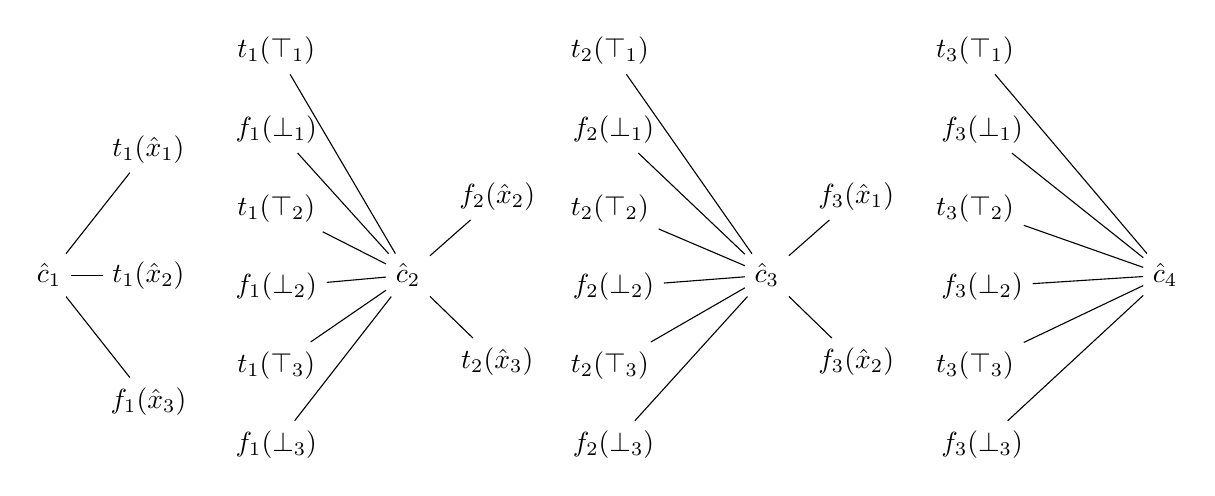
\begin{tikzpicture}[node distance=.3cm]

\node(c1){$\hat{c}_1$};

\node[right =.4cm of c1] (t1x2) {$t_1(\hat{x}_2)$};
\node[above =1cm of t1x2] (t1x1) {$t_1(\hat{x}_1)$};
\node[below =1cm of t1x2] (f1x3) {$f_1(\hat{x}_3)$};

\draw [-] (c1) to (t1x2);
\draw [-] (c1) to (t1x1);
\draw [-] (c1) to (f1x3);


\node[right =.4cm of t1x1, yshift = 0.25cm] (f11) {$f_1(\bot_1)$};
\node[above =.4cm of f11] (t11) {$t_1(\top_1)$};
\node[below =.4cm of f11] (t12) {$t_1(\top_2)$};
\node[below =.4cm of t12] (f12) {$f_1(\bot_2)$};
\node[below =.4cm of f12] (t13) {$t_1(\top_3)$};
\node[below =.4cm of t13] (f13) {$f_1(\bot_3)$};

\node[right = 4cm of c1](c2){$\hat{c}_2$};

\draw [-] (c2) to (t11);
\draw [-] (c2) to (t12);
\draw [-] (c2) to (t13);
\draw [-] (c2) to (f11);
\draw [-] (c2) to (f12);
\draw [-] (c2) to (f13);

\node[right =.25cm of c2, yshift=1cm]  (f2x2) {$f_2(\hat{x}_2)$};
\node[below =1.5cm of f2x2] (t2x3) {$t_2(\hat{x}_3)$};

\draw [-] (c2) to (f2x2);
\draw [-] (c2) to (t2x3);

\node[right =3cm of f11] (f21) {$f_2(\bot_1)$};
\node[right =3cm of t11] (t21) {$t_2(\top_1)$};
\node[right =3cm of t12] (t22) {$t_2(\top_2)$};
\node[right =3cm of f12] (f22) {$f_2(\bot_2)$};
\node[right =3cm of t13] (t23) {$t_2(\top_3)$};
\node[right =3cm of f13] (f23) {$f_2(\bot_3)$};

\node[right = 4cm of c2](c3){$\hat{c}_3$};

\draw [-] (c3) to (t21);
\draw [-] (c3) to (t22);
\draw [-] (c3) to (t23);
\draw [-] (c3) to (f21);
\draw [-] (c3) to (f22);
\draw [-] (c3) to (f23);

\node[right =.25cm of c3, yshift=1cm] (f3x1) {$f_3(\hat{x}_1)$};
\node[below =1.5cm of f3x1] (f3x2) {$f_3(\hat{x}_2)$};

\draw [-] (c3) to (f3x1);
\draw [-] (c3) to (f3x2);

\node[right =3.4cm of f21] (f31) {$f_3(\bot_1)$};
\node[right =3.4cm of t21] (t31) {$t_3(\top_1)$};
\node[right =3.4cm of t22] (t32) {$t_3(\top_2)$};
\node[right =3.4cm of f22] (f32) {$f_3(\bot_2)$};
\node[right =3.4cm of t23] (t33) {$t_3(\top_3)$};
\node[right =3.4cm of f23] (f33) {$f_3(\bot_3)$};

\node[right = 4.5cm of c3](c4){$\hat{c}_4$};

\draw [-] (c4) to (t31);
\draw [-] (c4) to (t32);
\draw [-] (c4) to (t33);
\draw [-] (c4) to (f31);
\draw [-] (c4) to (f32);
\draw [-] (c4) to (f33);

\end{tikzpicture}


\caption{Pos, Neg and Connect for $E_{\Phi}$}
\label{fig:npexamplebig}
\end{figure}


\begin{figure}[ht]


\centering
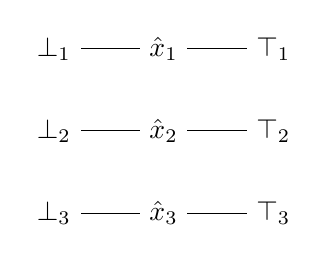
\begin{tikzpicture}[node distance=.75cm]

\node (x1) {$\hat{x}_1$};
\node [below =.5cm of x1] (x2) {$\hat{x}_2$};
\node [below =.5cm of x2] (x3) {$\hat{x}_3$};

\node [right = of x1] (t1) {$\top_1$};
\node [left = of x1] (f1) {$\bot_1$};

\draw [-] (x1) to (t1);
\draw [-] (x1) to (f1);

\node [right = of x2] (t2) {$\top_2$};
\node [left = of x2] (f2) {$\bot_2$};

\draw [-] (x2) to (t2);
\draw [-] (x2) to (f2);

\node [right = of x3] (t3) {$\top_3$};
\node [left = of x3] (f3) {$\bot_3$};

\draw [-] (x3) to (t3);
\draw [-] (x3) to (f3);

\end{tikzpicture}



\caption{Assignment for $E_{\Phi}$}
\label{fig:npassignment}
\end{figure}

\begin{figure}[ht]


\centering
\begin{tikzpicture}[node distance=1.5cm]

\node(c1){$\hat{c}_1$};

\node[right =.5cm of c1] (t1x1) {$t_1(\hat{x}_1)$};

\draw [-] (c1) to (t1x1);

\node[right =.5cm of t1x1] (t11) {$t_1(\top_1)$};

\draw [dashed] (t1x1) to (t11);

\node[right =.5cm of t11](c2){$\hat{c}_2$};

\draw [-] (c2) to (t11);

\node[right =.5cm of c2]  (f2x2) {$f_2(\hat{x}_2)$};

\draw [-] (c2) to (f2x2);

\node[right =.5cm of f2x2] (f22) {$f_2(\bot_2)$};

\draw [dashed] (f2x2) to (f22);

\node[right = .5cm of f22](c3){$\hat{c}_3$};

\draw [-] (c3) to (f22);

\node[right =.5cm of c3] (f3x2) {$f_3(\hat{x}_2)$};

\draw [-] (c3) to (f3x2);

\node[right =.5cm of f3x2] (f32) {$f_3(\bot_2)$};

\draw [dashed] (f3x2) to (f32);

\node[right =.5cm of f32](c4){$\hat{c}_4$};

\draw [-] (c4) to (f32);

\node [below =.5cm of f2x2] (x1) {$\hat{x}_1$};
\node [below =.5cm of x1] (x2) {$\hat{x}_2$};
\node [below =.5cm of x2] (x3) {$\hat{x}_3$};

\node [right = of x1] (t1) {$\top_1$};

\draw [-] (x1) to (t1);

\node [left = of x2] (f2) {$\bot_2$};

\draw [-] (x2) to (f2);

\node [right = of x3] (t3) {$\top_3$};

\draw [-] (x3) to (t3);

\end{tikzpicture}


\caption{Explanation of $(\hat{c}_1,\hat{c}_4)$}
\label{fig:npexplanation}
\end{figure}

\end{example}


\begin{lemma}[Characterization of explanations]
\label{lemma:charexpl}

Let $\Phi$ be a propositional logic formula in conjunctive normal form with $n$ clauses and $m$ variables.
For every subset $E$ of $E_{\Phi}$, $E \models \hat{c}_1 \thickapprox \hat{c}_{n+1}$ if and only if for every $i = 1,\ldots,n$ there is a $j = 1,\ldots,m$ such that $T_{ij} \subseteq E$ or $F_{ij} \subseteq E$.

\end{lemma}

\begin{proof}

Suppose that for every $i = 1,\ldots,n$ there is a $j = 1,\ldots,m$ such that $T_{ij} \subseteq E$ or $F_{ij} \subseteq E$.
Clearly $T_{ij} \models \hat{c}_i \thickapprox t_i(\hat{x}_j)$ and $T_{ij} \models t_i(\top_j) \thickapprox \hat{c}_{i+1}$. 
Since $(\hat{x}_j,\top_j) \in E$, the fact $E \models t_i(\hat{x}_j) \thickapprox t_i(\top_j)$ follows by an application of the compatibility axiom.
Using the transitivity of congruence relations, it follows that $T_{ij} \models \hat{c}_i \thickapprox \hat{c}_{i+1}$.
Similarly it can be shown that $F_{ij} \models \hat{c}_i \thickapprox \hat{c}_{i+1}$.
Therefore it follows from the assumption that $E \models \hat{c}_i \thickapprox \hat{c}_{i+1}$ for every $i = 1,\ldots,n$.
Using transitivity again, it follows that $E \models \hat{c}_1 \thickapprox \hat{c}_{n+1}$.

\noindent We show the other implication of the equivalence by induction on $n$.
\begin{paragraph}{Induction Base $n = 1$:}

Suppose that $E \models \hat{c}_1 \thickapprox \hat{c}_{2}$. %, which implies $\hat{c}_2 \in [\hat{c}_1]_E$.
Since $\hat{c}_1$ is a constant, the compatibility axiom can not be applied to extend the congruence class of $\hat{c}_1$ beyond the singleton $\{\hat{c}_1\}$.
Therefore in order to satisfy $E \models \hat{c}_1 \thickapprox u$ with $u \neq \hat{c}_1$ there has to be an equation $(\hat{c}_1, u) \in E$ for some term $u$.
Since $E \subseteq E_{\Phi}$, the only possible such equations are $(\hat{c}_1, t_1(\hat{x}_j))$ and $(\hat{c}_1, f_1(\hat{x}_j))$ for some $j$.
The only equations in $E$ involving terms with the function symbols $t_1$ and $f_1$ are $(\hat{c}_1, t_1(\hat{x}_j)), (t_1(\top_j),\hat{c}_2)$ and $(\hat{c}_1, f_1(\hat{x}_j)), (f_1(\bot_j),\hat{c}_2)$ for some $j$.
Therefore in order to satisfy $E \models \hat{c}_1 \thickapprox u$ such that $u$ is neither the constant $\hat{c}_1$, nor some term $t_1(\hat{x}_j), f_1(\hat{x}_j)$, it is necessary that $E \models t_1(\hat{x}_j) \thickapprox t_1(\top_j)$ and $(\hat{c}_1, t_1(\hat{x}_j)) \in E$ or $E \models f_1(\hat{x}_j) \thickapprox f_1(\bot_j)$ and $(f_1(\bot_j),\hat{c}_2) \in E$ for some $j$.
The conditions can only be satisfied with equations of $E_{\Phi}$ if $\{(\hat{c}_1, t_1(\hat{x}_j)), (\hat{x}_j,\top_j)\} \subseteq E$ or $\{(\hat{c}_1, f_1(\hat{x}_j), (\hat{x}_j,\bot_j)\} \subseteq E$ respectively.
%Similarly $t \in [\hat{c}_1]_E$ such that $t$ is neither $\hat{c}_1$ nor a term with the function symbol $t_1$ or $f_1$, for some $j$ $(t_1(\top_j),\hat{c}_2) \in E$ and 
From a similar argumentation about the equations involving $\hat{c_2}$ and $t_1(\top_j)$ or $f_1(\bot_j)$ it follows that either $T_{1j} \subseteq E$ or $F_{1j} \subseteq E$ for some $j$.
\end{paragraph}

\begin{paragraph}{Induction Hypothesis:} For every subset $E$ of $E_{\Phi}$, $E \models \hat{c}_1 \thickapprox \hat{c}_{n}$ if and only if for every $i = 1,\ldots,n-1$ there is a $j = 1,\ldots,m$ such that $T_{ij} \subseteq E$ or $F_{ij} \subseteq E$.
\end{paragraph}

\begin{paragraph}{Induction Step:}
Suppose that $E \models \hat{c}_1 \thickapprox \hat{c}_{n+1}$.\\
Similarly to the argumentation in the induction base, the only equations in $E_{\Phi}$ involving $\hat{c}_{n+1}$ are of the form $(t_n(\top_j),\hat{c}_{n+1})$ and $(f_n(\bot_j),\hat{c}_{n+1})$.
The only possibility to enrich the congruence class of $\hat{c}_{n+1}$ with terms other than $\hat{c}_{n+1}$ and those of the form $t_n(\top_j)$ and $f_n(\bot_j)$, 
is that for some $j$, $(\hat{x}_j,\top_j) \in E$ or $(\hat{x}_j,\bot_j) \in E$ and subsequently also $(\hat{c}_n,t_n(\hat{x}_j)) \in E$ or $(\hat{c}_n,f_n(\hat{x}_j)) \in E$.
Thus $T_{nj} \subseteq E$ or $F_{nj} \subseteq E$ and as a consequence $E \models \hat{c}_n \thickapprox \hat{c}_{n+1}$.
Using transitivity $E \models \hat{c}_1 \thickapprox \hat{c}_{n+1}$ and $E \models \hat{c}_n \thickapprox \hat{c}_{n+1}$ imply $E \models \hat{c}_1 \thickapprox \hat{c}_n$ and from the induction hypothesis it follows that  $T_{ij} \subseteq E$ or $F_{ij} \subseteq E$ for every $i = 1,\ldots,n-1$.
\end{paragraph}

\end{proof}

\begin{lemma}[NP- hardness]
\label{lemma:nphardness}
The short explanation decision problem is NP- hard.

\end{lemma}

\begin{proof}

We reduce SAT to the short explanation decision problem.
SAT is a well known NP-complete problem \cite{Biere2009}.
Let $\Phi$ be a propositional formula in conjunctive normal form with clauses $C_1,\ldots,C_n$ and variables $x_1,\ldots,x_m$.
Let $C_{n+1},\ldots,C_{n+m}$ be the tautological clauses $\{x_1, \neg x_1\},\ldots,\{x_m,\neg x_m\}$.
Clearly $\Phi$ is satisfiable if and only if $\Phi' = \{C_1,\ldots,C_{n+m}\}$ is satisfiable.
We will show that $\Phi'$ is satisfiable if and only if there exists $E \subseteq E_{\Phi'}$ such that $E \models \hat{c}_1 \thickapprox \hat{c}_{n+m+1}$ and $|E| \leq 2n + 3m$.

\emph{Suppose} $\Phi'$ is satisfiable and let $\mathcal{I}$ be a satisfying assignment.\\
For every clause $C_i$ there is a literal $\ell_i \in C_i$, such that $\mathcal{I} \models \ell_i$.
For every $i = 1,\ldots,n+m$ we set $E_i:= T_{ij}$ if $\ell_i = x_j$ and $E_i:= F_{ij}$ if $\ell_i = \neg x_j$.
From $\ell_i \in C_i$ follows $E_i \subseteq E_{\Phi'}$.
Let $E = \bigcup_i^n E_i$ then from Lemma \ref{lemma:charexpl} and the transitivity of the congruence relations follows $E \models \hat{c_1} \thickapprox \hat{c_{n+m+1}}$.
What remains to show is that $|E| \leq 2n + 3m$.
Since the sets $Pos, Neg$ and $Connect$ in the definition of $E_{\Phi'}$ are pairwise disjoint, for $i \neq j$ $E_i \cap E_j \subseteq \{(\hat{x}_j,\top_j),(\hat{x}_j,\bot_j) \mid j = 1,\ldots,m\}$.
Therefore $E$ involves exactly $2(n+m)$ equations of $Pos, Neg$ and $Connect$.
By construction of the sets $E_i$ and the clauses $C_{n+1},\ldots,C_{n+m}$ there is no $j = 1,\ldots,m$ such that $(\hat{x}_j,\top_j) \in E$ and $(\hat{x}_j,\bot_j) \in E$.
Therefore $E$ involves $m$ equations of set $Assignment$ in the definition of $E_{\Phi'}$.
Overall we have $|E| = 2n + 3m$.

\emph{Suppose} there exists $E \subseteq E_{\Phi'}$, $E \models \hat{c}_1 \thickapprox \hat{c}_{n+m+1}$ and $|E| \leq 2n + 3m$.\\
We will show that $\mathcal{I} = \{\hat{x}_j \mid (\hat{x}_j,\top_j) \in E\}$ is a satisfying assignment for $\Phi'$.
Let $i = 1,\ldots,n+m$ be an arbitrary clause index.
From $E \models \hat{c}_1 \thickapprox \hat{c}_{n+m+1}$ and Lemma \ref{lemma:charexpl} follows $T_{ij} \subseteq E$ or $F_{ij} \subseteq E$ for some $j=1,\ldots,m$.
Assume $T_{ij} \subseteq E$ for some $j = 1,\ldots,m$.
$E \subseteq E_{\Phi'}$ implies that $x_j$ appears positively in $C_i$. 
By definition of $\mathcal{I}$, $\mathcal{I} \models x_j$ and therefore $\mathcal{I} \models C_i$.
If $T_{ij} \nsubseteq E$ for all $j = 1,\ldots,m$, then $F_{ij} \subseteq E \subseteq E_{\Phi'}$, which implies that $x_j$ appears negatively in $C_i$, $x_j \notin \mathcal{I}$ and therefore $\mathcal{I} \models C_i$. Since $i$ was arbitrary we conclude $\mathcal{I} \models \Phi'$.

\end{proof}

\begin{lemma}[In NP]
\label{lemma:innp}
The short explanation decision problem is in NP.

\end{lemma}
\begin{proof}

Explanations are subsets of the input equations, therefore they are clearly polynomial in the problem size.
The congruence of two terms, i.e. verifying that a subset is actually an explanation, can be decided in $O(n \log(n))$ using for example the congruence closure algorithm presented in Section \ref{sec:algorithm}.

\end{proof}

Lemma \ref{lemma:nphardness} and \ref{lemma:innp} establish the main result of this section.

\begin{theorem}[NP - completeness]

The short explanation decision problem is NP- complete.

\end{theorem}

\section{Explanation Producing Congruence Closure}
\label{sec:algorithm}
%
In this section we present a congruence closure algorithm that is able to produce explanations.
The algorithm is a mix of the approaches of the algorithms presented in \cite{Fontaine2004} and \cite{Nieuwenhuis2005,Nieuwenhuis2007}.
The basic structure of the algorithm is inherited from \cite{Fontaine2004}, which itself inherits its structure from the algorithm of Nelson and Oppen \cite{Nelson1980}.
The technique to store and deduce equalities of compound terms is inspired by \cite{Nieuwenhuis2005,Nieuwenhuis2007}.
Additionally the proof forest structure described below was proposed by \cite{Nieuwenhuis2005,Nieuwenhuis2007}.

Before we describe the algorithm, we discuss two technical concepts that are important aspects of our congruence closure algorithm.

\subsubsection*{Curryfication and Abstract Congruence Closure}
\label{subsec:algorithms_preliminaries}

Our congruence closure algorithm operates on terms in curryfied form.
Such terms use a single binary function symbol to represent general terms.
More formally, let $\mathcal{F}$ be a finite set of functions with a designated binary function symbol $f \in \mathcal{F}$ and let every other function symbol in $\mathcal{F}$ be a constant.
A term w.r.t. a signature of this form is in \emph{curryfied form}.

It is possible to uniquely translate a general set of terms $\mathcal{T}^{\Sigma}$ with signature $\Sigma = \langle \mathcal{F},arity \rangle$ into a set of terms in curryfied form $\mathcal{T'}^{\Sigma'}$.
The new signature $\Sigma'$ is obtained from $\Sigma$ by setting $arity$ to zero for every function symbol in $\mathcal{F}$ and introducing the designated binary function symbol $f$ to $\mathcal{F}$.
The translation of a term $t \in \mathcal{T}^{\Sigma}$ is given in terms of the function $curry$.

$$
curry(t) = \Big\{
\begin{array}{ll}
	t & \text{ if } t \text{ is a constant }\\
	f(\ldots (f(f(g,curry(t_1)),curry(t_2)))\ldots,curry(t_n)) &\text{ if } t = g(t_1,\ldots, t_n)
\end{array}
$$

The idea of currying was introduced by M. Sch\"onfinkel \cite{Schoenfinkel1924} in 1924 and independently by Haskell B. Curry \cite{Curry1958} in 1958, who lends his name to the concept.
Currying is not restricted to terms.
The general idea is to translate functions of type $A \times B \rightarrow C$ into functions of type $A \rightarrow B \rightarrow C$.
There is a close relation between currying and lambda calculus \cite{Church1936}.
In the simplest form of lambda calculus, every function is in curried form.
For an introduction to lambda calculus, including currying in terms of lambda calculus and its relation to functional programming we refer the reader to \cite{Barendregt1997}.

The benefit of working with terms in curryfied form is an easier and cleaner congruence closure algorithm, while maintaining best known runtime for congruence closure algorithms of $O(n \log(n))$.
Terms in curryfied form simplify the algorithm, because case distinctions on terms are much simpler.
Such a term is either a constant or a compound term of the form $f(a,b)$, where $a$ and $b$ are terms in curryfied form.
In general, terms can have different leading function symbols and their arities (for which possibly there is no known bound) have to be taken into account.
Cleaner algorithms are not only easier to implement, but should also improve the practical runtime for similar reasons.
Additionally, working with terms in curryfied form replaces tedious preprocessing steps, for example transformation to a graph of outdegree 2 \cite{Downey1980},that are necessary for other algorithms to achieve the optimal running time.

Recently so called abstract congruence closure algorithms have been proposed and shown to be more efficient than traditional approaches \cite{Bachmair2000}.
The idea of abstract congruence closure is to introduce new constants for non constant terms.
Doing so, all equations the algorithm has to take into account are of the form $(c,d)$ and $(c, f(a,b))$, where $a,b,c,d$ are constants.

Our method does not use the idea of abstract congruence closure.
We found that using currying is enough to obtain an algorithm with optimal running time and no tedious preprocessing steps.
The reason why we did not go for abstract congruence closure is, that we do not want to have the overhead of introducing and eliminating fresh constants.
In the context of proof compression, our congruence closure algorithm will be applied to relatively small instances very often.
We could introduce the extra constants for the whole proof before processing, but would still have to remove them from explanations every time we produce a new subproof.
It would be interesting to investigate, whether our intuition in that regard is right, or if it pays off to deal with extra constants.

\cite{Nieuwenhuis2005,Nieuwenhuis2007} describes an explanation producing abstract congruence closure algorithm, 
whereas \cite{Fontaine2004} proposes a traditional algorithm without currying and extra constants.
By choosing to work with terms in curryfied form, but without extra constants, our algorithm is a middle ground between the two algorithms.

\subsubsection*{Immutable Data Structures}

Most of the data structures presented in the following section are defined in terms of mathematical functions.
This is not by coincidence and our congruence closure algorithm can easily be translated to an implementation in a functional programming language.
Furthermore, all data structures can be implemented immutable.
An immutable data structure is one that never changes its internal state after its creation.
When alternating the information stored in the data structure, a new object with the new information is constructed.
The old object remains intact.

A side effect of a method is a modification of an object that is not the returned value of the method.
Such side effects often lead to bugs, since the method can not be used as a black box anymore.
An example for a side effect is the modification of the representative of a term in the congruence closure algorithm presented in \cite{Fontaine2004} and its effect on what is called signature table in this work.
Using immutable data structures prohibits side effects by design.
Furthermore immutable data structures allow to maintain internal correctness much easier.
For example, in the Skeptik tool resolution nodes are stored in an immutable fashion.
Modifying the premise of a node does not have an effect on the node itself, since its premise remains to be the old version.
Therefore the correctness of a resolution proof, once established when creating a proof is maintained without any further actions.
Functional programming languages almost exclusively use immutable data structures and often it is not easy or impossible to translate an imperative description of an algorithm into functional programming.
Sometimes it is possible, but not with the same runtime.

Immutable data structures also have some downsides.
The impossibility of changing internal structures often makes it hard to maintain certain structures without a lot of extra effort.
One simple example is that of a linked list.
Suppose such a linked list is implemented in such a way that every element of the list internally has a pointer to the next element in the list.
When modifying the first element of the list in some fashion, the pointer of the second element has to be set to the new version of the first one.
Since this requires to produce a new version of the second element as well, also the pointer of the third element has to be updated and so on. 
Eventually, every element of the list will have to be updated.
A mutable linked list would simply alter the internal state of the first element and leave everything else as it is.
Some algorithms and their optimal runtime depend the runtime of such simple data structures, that are very hard or impossible to achieve in an immutable fashion.
However, sometimes tricky data structures like the zipper were invented which help to overcome these problems.

\subsubsection*{Congruence structure}

We call the underlying data structure of our congruence closure algorithm a \emph{congruence structure}.
A congruence structure for set of terms $\mathcal{T}$ is a collection of the following data structures.
The set $\mathcal{E} = \mathcal{T} \times \mathcal{T} \cup \{\smiley\}$ is the set of \emph{extended equations}.
The symbol $\smiley$ serves as a placeholder for deduced equalities that have to be explained in terms of input equations.

\begin{itemize}
	\item Representative $r: \mathcal{T} \rightarrow \mathcal{T}$
	\item Congruence class $[.]: \mathcal{T} \rightarrow 2^\mathcal{T}$
	\item Left neighbors $N_l: \mathcal{T} \rightarrow 2^\mathcal{T}$
	\item Right neighbors $N_r: \mathcal{T} \rightarrow 2^\mathcal{T}$
	\item Lookup table $l: \mathcal{T} \times \mathcal{T} \rightarrow \mathcal{T}$
	\item Congruence graph $g$
	\item Queue $\mathcal{Q}$ of pairs of terms
	\item Current explanations $\mathcal{M}: \mathcal{T} \times \mathcal{T} \rightarrow \mathcal{E}$
\end{itemize}

The representative is one particular term of a class of congruent terms.
It is used to identify whether two terms are in the same congruence class and the data structures ($l, N_l$ and $N_r$) used for detecting deduced equalities are kept updated only for representatives.
The congruence class structure represents a set of pairwise congruent terms.
It is used to keep track which representatives have to be updated when merging the classes of two terms.
The structures left $N_l$ (resp. right $N_r$) neighbor  keeps track of the respective other terms in compound terms.
The information is only used for representatives (i.e. terms in the target of $r(.)$).
Furthermore right and left neighbors always only contain one term per congruence class (which is not necessarily the representative of that class).
The lookup table is used to keep track of all compound terms in the congruence structure and to merge classes of compound terms, which arguments are congruent.
For example if the terms $f(a,b),f(c,d)$ were inserted and the representatives are such that $r(a) = r(c), r(b) = r(d)$, then $N_r(r(a)) = \{d\}$, $N_l(r(d)) = \{a\}$ and $l(r(a),r(b)) = f(a,b)$.
The elements in the respective sets serve as pointers to their representatives, therefore it does not matter whether for example $N_r(r(a)) = \{d\}$ or $N_r(r(a)) = \{b\}$.
In Section \ref{sec:congruenceclosurealgorithm} we explain how these structures are modified and used in detail.
The congruence graph (explained in detail in Section \ref{sec:congruencegraph}) stores the derived equalities in a structured way, that allows to create explanations for a given pair of terms.
Edges are added to the graph in a lazy way, meaning that they are buffered and only actually entered into the graph when demanded.
The queue $\mathcal{Q}$ keeps track of the order in which edges should be added to the graph.
The function $\mathcal{M}$ stores explanations if they exist for buffered edges.
The idea will be explained in detail in Section \ref{sec:proofproduction}.
We call the unique congruence structure for $\mathcal{T} = \emptyset$ the \emph{empty congruence structure}.

\FloatBarrier

\subsubsection*{Congruence closure algorithm}
\label{sec:congruenceclosurealgorithm}
In this section we present our explanation producing congruence closure algorithm and state and prove its properties.
Most importantly we show that the algorithm is sound and complete and has the best known asymptotic running time $O(n \log(n))$, where $n$ is the number of terms in the input.
Computing the congruence closure of some set of equations $E$ is done by adding all equations to an ever growing congruence structure, which initially is empty.
Since this has to be done in some order, we will often assume that $E$ is given as a sequence of equations rather than a set.
The pseudocode of most methods do not include return statements.
In fact every method implicitly returns a (modified) congruence structure or simply modifies a global variable, which is the current congruence structure.
Adding an equation to a congruence structure is done with the \texttt{addEquation} method, which is the only method that has to be visible to the user.
The method adds boths sides of the equation to the current set of terms using the \texttt{addNode} method and afterwards merges the classes of the two terms.
The \texttt{addNode} method enlarges the set of terms and detects deduced equalities.
The updates of the set of terms are not outlined explicitly, but are understood to happen implicitly.
Throughout this chapter we denote this implicit set of terms by $\mathcal{T}$.
The method \texttt{merge} initializes and guides the merging of congruence classes.
The actual merging is done by the method \texttt{union} by modifying the data structures.
The method does not only merge classes, but also searches for and returns deduced equalities.
The classes of the terms of these extra equalities are merged, if they are not equal yet.
The congruence classes are kept track of in a graph, maintaining important information for producing explanation and proofs.
We call such a graph Congruence Graph and explain them in a more detailed fashion in Section \ref{sec:congruencegraph}.
Edges, that reflect detected equalities, are not inserted into the graph right away, but stored in queue until the insertion is requested.
The reason for adding edges in a lazy way is to produce shorter explanations and proofs and will be explained and exemplified in Section \ref{sec:proofproduction}.

\begin{algorithm}[t]
\caption[.]{addEquation}
  \KwIn{equation $(s,t)$}
	
	addNode($s$) \\
	addNode($t$) \\
	merge($s, t, (s,t)$)
  
  \label{algo:addEquation}
\end{algorithm}


\begin{algorithm}[t]
	\caption[.]{addNode}
  \KwIn{term $v$}
	
	\If{$r$ is not defined for $v$}
		{$r(v) \leftarrow v$ \\
		$[v] \leftarrow \{v\}$ \label{initclass} \\
		$N_l(v) \leftarrow \emptyset$ \\
		$N_r(v) \leftarrow \emptyset$ \label{initrN} \\
		\If{$v$ is of the form $f(a,b)$}{
			addNode(a) \\
			addNode(b) \\
			\eIf{$l$ is defined for $(r(a),r(b))$ and $l(r(a),r(b)) \neq f(a,b)$ \label{line:ldefined}}{
				merge($l(r(a),r(b)),f(a,b),\smiley$) \label{addnodemerge} 
			}
			{
				$l(r(a),r(b)) \leftarrow f(a,b)$ \label{line:initl} \\ 
			}
			$N_l(r(b)) \leftarrow N_l(r(b)) \cup \{a\}$ \\
			$N_r(r(a)) \leftarrow N_r(r(a)) \cup \{b\}$ \label{modifyrN}\\
			%\KwAssert{Neighbours \nllabel{invariant:neig_add}} 
		 }
	}
	
  
  \label{algo:addNode}
\end{algorithm}


\begin{algorithm}[t]
\caption[.]{merge}
  \KwIn{term $s$}
	\KwIn{term $t$}
	\KwIn{extended equation $eq$}
	
	\If{$r(s) \neq r(t)$}{
		$c \leftarrow \{(s,t)\}$ \\
		$eq \leftarrow (s,t)$ \\
		\While{$c \neq \emptyset$}{
			Let $(u,v)$ be some element in $c$ \\
			$c \leftarrow c \setminus \{(u,v)\} \cup union(u,v)$ \\
			lazy\_insert$(u,v,eq)$ \label{graphinsert} \\
			$eq \leftarrow null$
		}
	}
  %\KwAssert{$r(s) = r(t)$ \nllabel{assertion:merge_rep}}
  \label{algo:merge}
\end{algorithm}


\begin{algorithm}[t]
\caption[.]{union}
  \KwIn{term $s$}
	\KwIn{term $t$}
	\KwOut{a set of deduced equalities}
	
	\eIf{$[r(s)] \geq [r(t)]$}{
		$(u,v) \leftarrow (s,t)$ \label{reverse1} 
	}
	{
		$(u,v) \leftarrow (t,s)$ \label{reverse2} 
	}
	$d \leftarrow \emptyset$ \\
	\For{every $x \in N_l(r(v))$ \label{startlN}}{
		$l_v \leftarrow l(r(x),r(v))$ \label{accessl1} \\
		\eIf{$r(x) = r(v)$}{
			$new\_left \leftarrow r(u)$
		}{
			$new\_left \leftarrow r(x)$
		}
		\eIf{$l$ is defined for $(new\_left,r(u))$}{
			$l_u \leftarrow l(new\_left,r(u))$ \\
			\eIf{$r(l_u) \neq r(l_v)$}{
				$d \leftarrow d \cup \{(l_u,l_v)\}$ \label{deduceEq1} 
			}
			{
				$N_l(r(v)) \leftarrow N_l(r(v)) \setminus \{x\}$
			}
		}
		{
			$l(new\_left,r(u)) \leftarrow l_v$ \label{changel1} 
		}
	\label{stoplN}}
	\For{every $x \in N_r(r(v))$ \label{startrN}}{
		$l_v \leftarrow l(r(v),r(x))$ \label{accessl2} \\
		\eIf{$r(x) = r(v)$}{
			$new\_right \leftarrow r(u)$
		}{
			$new\_right \leftarrow r(x)$
		}
		\eIf{$l$ is defined for $(r(u),new\_right)$}{
			$l_u \leftarrow l(r(u),new\_right)$ \\
			\eIf{$r(l_u) \neq r(l_v)$}{
				$d \leftarrow d \cup \{(l_u,l_v)\}$ \label{deduceEq2} 
			}
			{
				$N_r(r(v)) \leftarrow N_r(r(v)) \setminus \{x\}$
			}
		}
		{
			$l(r(u),new\_right) \leftarrow l_v$ \label{changel2}
		}
	\label{stoprN}}
	$[r(u)] \leftarrow [r(u)] \cup [r(v)]$ \label{changeclass} \\
	\For{every $x \in [r(v)]$}{
		$r(x) \leftarrow r(u)$ \label{changerep} 
	}
	$N_l(r(u)) \leftarrow N_l(r(u)) \cup N_l(r(v))$ \\
	$N_r(r(u)) \leftarrow N_r(r(u)) \cup N_r(r(v))$ \label{modifyrN2} \\
	%\KwInvariant{Neighbours \nllabel{invariant:neig_union}} \\
	%\KwAssert{$r(s) = r(t)$ \nllabel{assertion:union_rep}}
	\Return $d$
  \label{algo:union}
\end{algorithm}



\begin{algorithm}[t]
\caption[.]{lazy\_insert}
  \KwIn{term $s$}
	\KwIn{term $t$}
	\KwIn{extended equation $eq$}
	%\KwGlobal{Queue of tuples of terms $\mathcal{Q}$}
	%\KwGlobal{Map of tuples of terms to equation $\mathcal{M}$}
	
	\eIf{$\mathcal{M}$ is set for $(s,t)$}{
		\If{$eq \neq \smiley$}{
			$\mathcal{M}(s,t) \leftarrow (s,t)$
		}
	}{
		$\mathcal{Q} \leftarrow \mathcal{Q}.enqueue(s,t)$ \\
		$\mathcal{M}(s,t) \leftarrow eq$ 
	}
  
  \label{algo:lazyinsert}
\end{algorithm}


\begin{algorithm}[t]
\caption[.]{lazy\_update}
	%\KwIn{congruence graph $g$}
	%\KwGlobal{Queue of tuples of terms $\mathcal{Q}$}
	%\KwGlobal{Map of tuples of terms to equation $\mathcal{M}$}
	
	\While{$\mathcal{Q}$ is not empty}{
		$(u,v) \leftarrow \mathcal{Q}.dequeue$\\
		$eq \leftarrow \mathcal{M}(u,v)$ \\
		$g.insert(u,v,eq)$
	}
  
  \label{algo:lazyupdate}
\end{algorithm}



In the following pages, we will provide some invariants that are essential for proving the properties of the algorithm.
The invariants hold when initializing the respective data structures and before and after every insertion of an equation via the \texttt{addEquation} method.

\begin{invariant}[Class]

For every $s \in \mathcal{T}$ and every $t \in [r(s)]$, $r(t) = r(s)$.

\label{invar:class}
\end{invariant}
%{\color{blue} For all invariants I might need to be more specific as to when exactly they should old.}
\begin{proof}

Clearly the invariant is true when intializing $[s]$ in line \ref{initclass} of \texttt{addNode}.

The only other point in the code that changes $[s]$ is line \ref{changeclass} of union.
Suppose the class of $u$ is enlarged by the class of $v$ in union and suppose the invariant holds before the union for those terms.
Before the update of $[r(u)]$ the representative of every term in $[r(v)]$ is set to $r(u)$.
Therefore the invariant remains valid after the update.

\end{proof}

\begin{invariant}[Lookup]

The lookup structure $l$ is defined for a pair of terms $(s,t)$ if and only if there is a term $f(a,b) \in \mathcal{T}$ such that $r(a) = r(s)$ and $r(b) = r(t)$.

\end{invariant}

\begin{proof}

Suppose $l$ is defined for some pair of terms $(s,t)$.
The value of $l(s,t)$ is set either in lines \ref{changel1} or \ref{changel2} of \texttt{union} or in line \ref{line:initl} of \texttt{addNode}.
In the latter case, $l$ is set to $f(a,b)$ for the tuple $(r(a),r(b))$ and therefore the invariant holds at this point.
For changes to $r(a)$ or $r(b)$ in union the one implication of the invariant remains valid in case $l$ is defined for the new representatives, or $l$ is set for an additional pair of terms in lines \ref{changel1} or \ref{changel2}.
In case $l$ is set to $(new\_left,r(u))$ or $(r(u),new\_right)$ in union, there is an $l$-entry $l_v$ for which the invariant held before the union.
The changes in representatives of $x$ are reflected by $new\_left$ and $new\_right$, while the representative of $v$ is changed to $r(u)$.
The new entry for $l$ therefore respects the implication of the invariant.

To show the other implication, let $f(a,b) \in \mathcal{T}$.
The term $f(a,b)$ is entered with the \texttt{addEquation} method and subsequently via the \texttt{addNode} method.
For compound terms lines \ref{line:ldefined} and \ref{line:initl} assert that $l$ is defined for $(r(a),r(b))$.
All changes to $r(a)$ or $r(b)$ must happen in \texttt{union} and they are reflected by matching updates to the $l$ structure.

\end{proof}


\begin{invariant}[Neighbours]

For every $s \in \mathcal{T}$, every $t_r \in N_r(r(s))$ and $t_l \in N_l(r(s))$, $l$ is defined for $(r(s),r(t_r))$ and $(r(t_l),r(s))$.

\end{invariant}

\begin{proof}

We show the result for the structure $N_r$.
The result about $N_l$ can be obtained analogously.
Since $N_r$ is initialized with the empty set in line \ref{initrN} of \texttt{addNode}, the invariant clearly holds initially.
To show that the invariant always holds, it has to be shown that all modifications of $r$ and $N_r$ preserve the invariant.
The structure $l$ is not modified after initialization.
Line \ref{modifyrN} of \texttt{addNode} adds $b$ to $N_r(r(a))$ and the four lines before that addition show that $l$ is defined for $(r(a),r(b))$.
Union modifies $N_r$ in such a way that it adds all right neighbors of some representative $r(v)$ to $N_r(r(u))$.
Lines \ref{startrN} to \ref{stoprN} make sure that $l$ is defined for all these right neighbors.
Updates of $r$ in \ref{changerep} are always followed by corresponding updates to $N_r$.

\end{proof}

A consequence of this invariant is the fact that, that for every term $t \in \mathcal{T}$ of the form $f(a,b)$, $l$ is defined for $(r(a),r(b))$.

\begin{proposition}[Sound- \& Completeness]

Let $r(.)$ be the representative mapping obtained by adding equations $E = \langle (u_1,v_1), \ldots, (u_n,v_n) \rangle $ to the empty congruence structure.
For every $s,t \in \mathcal{T}_E$: $E \models s \thickapprox t$ if and only if $r(s) = r(t)$.

\end{proposition}

\begin{proof}
\textbf{Completeness}

\noindent We show that from $E \models s \thickapprox t$ follows $r(s) = r(t)$ by induction on $n$.

\begin{itemize}
\item \textbf{Induction Base} $n=1$: $E \models s \thickapprox t$ implies either $s = t$ or $\{u_1,v_1\} = \{s,t\}$.
In the first case $r(s) = r(t)$ is trivial. 
In the second case, the claim follows from the fact that, when $(u_1,v_1)$ is entered, union is called with arguments $s$ and $t$.
After this operation $r(s) = r(t)$.

\item \textbf{Induction Hypothesis}: For every sequence of equations $E_n$ with $n$ elements and every $s,t \in \mathcal{T}_{E_n}$: $E_n \models s \thickapprox t$ then $r(s) = r(t)$.

\item \textbf{Induction Step}: Let $E = \langle (u_1,v_1), \ldots, (u_{n+1},v_{n+1}) \rangle$ and $E_n = \langle (u_1,v_1), \ldots, (u_n,v_n) \rangle$.
There are two cases: $E_n \models s\thickapprox t$ and $E_n \nvDash s\thickapprox t$.
In the former case, the claim follows from the induction hypothesis, the Invariant class and the fact that union always changes representatives for all elements of a class.
We still have to show the claim in the latter case.
We write $E \models_n u \thickapprox v$ as an abbreviation for $E_n \nvDash u \thickapprox v$ and $E \models u \thickapprox v$.
We show the claim ($r(s) = r(t)$) by induction on the structure of the terms $s$ and $t$.

\begin{itemize}
\item \textbf{Induction Base} $s$ or $t$ is a constant and therefore transitivity reasoning was used to derive $E \models_n s \thickapprox t$.
In other words, there are $m$ terms $t_1,\ldots,t_m$ such that $s = t_1$, $t = t_m$ and for all $i = 1,\ldots,m-1: E \models_n t_i \thickapprox t_{i+1}$.
We prove by yet another induction on $m$ that $r(t_1) = r(t_m)$.
\begin{itemize}
\item \textbf{Induction Base} $m = 2$. It has to be the case (up to swapping $u_{n+1}$ with $v_{n+1}$), that $E_n \models s \thickapprox u_{n+1}$ and $E_n \models t \thickapprox v_{n+1}$, and the outmost induction hypothesis implies $r(s) = r(u_{n+1})$ and $r(t) = r(v_{n+1})$.
Therefore it follows from Invariant Class, that after the call to union for $(u_{n+1},v_{n+1})$ it is the case that $r(t_1) = r(t_2)$.

\item \textbf{Induction Step}: Suppose that the claim holds for all sequences of length $m \in \mathbb{N}$, for $m+1$ the claim follows from a simple application of the transitivity axiom, since $t_1,\ldots,t_m$ and $t_2,\ldots,t_{m+1}$ are both sequences of length $m$.
\end{itemize}
\item \textbf{Induction Step}: Suppose that $s = f(a,b)$ and $t = f(c,d)$.
There are two cases such that $E \models_n s \thickapprox t$ can be derived.
Using a transitivity chain, the claim can be shown just like in the base case.
Using the compatibility axiom, it has to be the case that $E \models_n a \thickapprox c$ and $E \models_n b \thickapprox d$ (in fact one of those can also be the case without the $n$ index).
The terms $a,b,c,d$ are of lower structure than $s$ and $t$.
Therefore it follows from the induction hypothesis that $r(a) = r(c)$ and $r(b) = r(d)$.
The Invariants Neighbour and Lookup imply that either $r(s) = r(t)$ or $(s,t)$ is added to $d$ in line \ref{deduceEq1} or line line \ref{deduceEq2} of union.
Subsequently union is called for $s$ and $t$, after which $r(s) = r(t)$ holds.
\end{itemize}
\end{itemize}

\noindent\textbf{Soundness}

\noindent For $s = t$ the claim follows trivially.
Therefore we show soundness in case $s \neq t$.
We show that from $r(s) = r(t)$ follows $E \models s \thickapprox t$ by induction on the number $m$ of calls to union induced by adding all equations of $E$ to the empty congruence structure, for all $s$ and $t$ that are arguments of some call to union.
The original claim then follows from Invariant Class, since only union modifies the $r$ structure and the fact that two terms are in the same class if and only if union was called for some elements in the respective classes.
%Notice that only union modifies $r$ after initialization.
%Therefore the proof investigates the changes made by union and the parameters it is called when adding equations to a congruence structure.
\begin{itemize}
\item \textbf{Induction Base} $m = 1$: $r(s) = r(t)$ implies $\{u_1,v_1\} = \{s,t\}$ and $E \models s \thickapprox t$ is trivial.
%Lines \ref{deduceEq1} and \ref{deduceEq2} do not induce any further unions, because no compound terms, that $s$ or $t$ could be a subterm of, are yet inserted in the congruence structure.

%Induction hypothesis: For every sequence of equations $E_n$ with $n$ elements and every $s,t \in \mathcal{T}_{E_n}$: $r(s) = r(t)$ after adding all $n$ equations to the empty congruence structure then $E_n \models s \thickapprox t$.

\item \textbf{Induction Hypothesis}: For every $k < m$, if a set of equations $F$ induces $k$ calls to union, then from $r(s) = r(t)$ follows $F \models s \thickapprox t$ for all terms $s,t$ that are arguments of some call to union.

\item \textbf{Induction Step}: Suppose $E = \langle (u_1,v_1), \ldots, (u_n,v_n) \rangle$ induces $m$ calls to union with arguments $(h_1,g_1),\ldots,(h_m,g_m)$.
The subsequence $E_n = \langle (u_1,v_1), \ldots, (u_{n-1},v_{n-1}) \rangle$ induced the first $k$ calls to union for some $n-1 \leq k < m$.
In other words, adding $(u_n,v_n)$ to the congruence structure induces $m-k-1$ calls to union with arguments $(h_{k+1},g_{k+1}),\ldots,(h_m,g_m)$.
The pair $(h_{k+1},g_{k+1})$ is either an original input equation, or a deduced equality from line \ref{addnodemerge} of \texttt{addNode}.
In both cases $E \models h_{k+1} \thickapprox g_{k+1}$, which is trivial in the former case.
In the latter case $h_{k+1} = f(a,b)$ and $g_{k+1} = f(c,d)$ for some terms $a,b,c,d$ and suppose $l(r(a),r(b)) = g_{k+1}$ (the other case that triggers line \ref{addnodemerge} $l(r(c),r(d)) = h_{k+1}$ is symmetric).
From the invariant Lookup follows $r(a) = r(c)$ and $r(b) = r(d)$.
Using the induction hypothesis we can see that $E \models h_{k+1} \thickapprox g_{k+1}$.

Let $j \in \{k+2,\ldots,m\}$.
The pair $(h_j,g_j)$ was inserted to $d$ in line \ref{deduceEq1} or \ref{deduceEq2} of \texttt{union} that was called with arguments $(h_i,g_i)$ with $i \in \{k+1,\ldots,j-1\}$.
From the Invariant Lookup follows that the terms are such that $h_i$ and $g_i$ are both subterms of $h_j$ or $g_j$.
Therefore, using induction on the structure of terms, the original induction hypothesis, Invariants Lookup and Neighbour and lines \ref{startlN} to \ref{stoprN} of \texttt{union}, it can be seen that for all pairs $(h_k,g_k)$ and all $k = l+1,\ldots,m$ it is the case that $E \models h_k \thickapprox g_k$.

%
%We show the induction step by another induction on $k-l$, i.e. the number of unions induced by adding $(u_n,v_n)$ to the congruence structure.
%Base case $k-l = 1$: Union is called for $(u_n,v_n)$ and the induces no further calls union.
%After the one call to union $r(u_n) = r(v_n)$ and clearly $E \models u_n \thickapprox v_n$.
%The fact that lines \ref{deduceEq1} and \ref{deduceEq2} of union do not induce any further calls to the method, together with the induction hypothesis and the invariants Lookup and Neighbour, imply that $E \models_n s \thickapprox t$ if and only if $s,t = \{u_n,v_n\}$.
%
%Induction step: Suppose adding $(u_n,v_n)$ induces $m$ calls to union with arguments $(h_{k-m},g_{k-m}),\ldots,(h_k,g_k)$.
%The last call to union has to be added 
%
%Adding the equation $(u_{n+1},v_{n+1})$ to the working congruence structure induces a sequence of $l$ calls to union with parameters $(h_1,g_1),\ldots,(h_l,g_l)$

%After initialization of $r$ only union modifies the structure.
%Adding $E$ to the empty congruence structure induces a sequence of calls to union with parameters $(u_1,v_1), \ldots , (u_n,v_n)$.
%We show by induction on $n$, that $E \models v_i \thickapprox u_i$
\end{itemize}
\end{proof}

\begin{proposition}[Runtime]
\label{prop:runtime}
Let $E$ be a set of equations such that $|\mathcal{T}_E| = n$.
Computing the congruence closure with our congruence closure algorithm takes worst-case time $O(n \log(n))$.

\end{proposition}

\begin{proof}

There are three loops in the method \texttt{union}, which are nested within the loop of \texttt{merge}.
These loops are clearly the dominating factor for runtime.
Lines \ref{reverse1} and \ref{reverse2} of \texttt{union} swap the arguments $s$ and $t$ in such a way, that always the congruence class of $v$ is smaller than the one of $u$.
Let $k$ be the size of the congruence class of $v$ before the union.
For every term in the congruence classes of $v$ and $u$ before the union, the size of their new congruence class after the union (set in line \ref{changeclass}) is at least $2*k$.
Furthermore, only representatives for terms in the old congruence class of $v$ are changed in line \ref{changerep}.
This implies that for every term, whenever its representative is changed in line \ref{changerep}, its congruence class doubles in the same execution of \texttt{union}.
The maximum size of a congruence class is $n$.
Therefore the representative of a single term is changed in line \ref{changerep} maximally $\log(n)$ times.
There are $n$ terms that can be changed, so line \ref{changerep} of \texttt{union} is executed at most $n \log(n)$ times.
Let $f(a,b)$ be the result of accessing $l$ in line \ref{accessl1}.
In the same call of \texttt{union} line \ref{changerep} changes the representative of $b$.
Since this this happens only $\log(n)$ times and there are at most $m < n$ compound terms, line \ref{accessl1} is executed at most $n \log(n)$ times.
The same holds for line \ref{accessl2} and all other lines in the respective loops.

\end{proof}


\FloatBarrier

\subsubsection*{Congruence Graph}
\label{sec:congruencegraph}
The most important feature of our congruence closure algorithm towards proof compression is explanation production.
For this purpose the input equations and deduced equalities have to be stored in a data structure that supports this feature.
We present two different such data structures.
Both structures store equalities in labeled graphs, which we call congruence graphs.
A node in such a graph represents a term and an edge between two nodes denotes that the represented terms are congruent w.r.t. the set of input equations.
A path in a congruence graph is a sequence of undirected, unweighted, labeled edges in the underlying graph.
The set of labels for both types of graphs is the set of extended equations $\mathcal{E}$ (i.e. equations and the placeholder \smiley).
The method \texttt{merge} adds edges to the graph via the \texttt{lazy\_insert} method, which eventually calls the \texttt{insert} method.
The \texttt{insert} method is different for the two presented structures.
After calling \texttt{insert} with arguments $s$ and $t$ it is guaranteed that there is a path in the congruence graph between $s$ and $t$.
In case they were not connected before the call, then there is an edge between $s$ and $t$ after the call.
The same can be assumed for \texttt{lazy\_insert} since edges that are added to the queue are never discarded and $s$ and $t$ are connected virtually.
The methods \texttt{insert} and \texttt{explain} are assumed to be attached to the data structures.
For example adding an edge to the data structure means adding it to the used congruence graph.

\begin{invariant}[Paths]

For terms $s, t$ holds $r(s) = r(t)$ if and only if there is a path in the congruence graph of the structure between $s$ and $t$.

\end{invariant}

\begin{proof}

In case $s = t$, the claim is trivial.
Therefore, we show the invariant for $s \neq t$ by an induction on $|[r(s)]|$.
%We show that there is a path between $s$ and $t$ in the congruence graph induction on $|[r(s)]|$. 
The proof relies on the invariant Class, which shows the consistency between classes and representatives.

\begin{itemize}
\item \textbf{Induction Base:} $[r(s)] = \{s\}$, i.e. $r(s) = r(t)$ is false for every term $t \neq s$.
We have to show that there is no edge $(s,t)$ for $t \neq s$ in the congruence graph.
Edges are only added to the congruence graph via the \texttt{lazy\_insert} method which is only called in \texttt{merge}.
Clearly \texttt{merge} does not call \texttt{union} for $s$ and some term $t \neq s$, since otherwise $t \in [r(s)]$.
Therefore \texttt{merge} also does not add an edge for $s$ and some term $t \neq s$ to the congruence graph.

\item \textbf{Induction Hypothesis:} For every term $s$ such that $|[r(s)]| \leq n$ and for every term $t \neq s$ it is the case that $r(s) = r(t)$ if and only if there is a path between $s$ and $t$ in the congruence graph.

\item \textbf{Induction Step:} Suppose $[r(s)]$ is an arbitrary class with cardinality $n+1$.
Then there are two terms $u,v \in [r(s)]$ such that \texttt{union} was called for $u$ and $v$.
Before the union $|[r(u)]|$ and $|[r(v)]|$ both were strictly smaller than $n+1$.
In case they both belong to the same class before the union, the claim follows trivially by the induction hypothesis, since existing paths are not removed by adding new edges to the graph.
Suppose $s \in [r(u)]$ and $t \in [r(v)]$, then by induction hypothesis there are paths $p_1$ between $s$ and $u$ and $p_2$ between $t$ and $v$.
Right after the union of $u$ and $v$, an edge is inserted between them, so $p_1$ concatenated with $(u,v)$ and $p_2$ is a path between $s$ and $t$.
In case one of the terms did not belong to one of the classes before the union, it does not belong to the merged class after the union.
Also there was no path between the two terms before and since the only addition paths are between elements of $[r(u)]$ and $[r(v)]$, there is no path between the terms after the union.
\end{itemize}

\end{proof}

\begin{invariant}[Deduced Edges]

For every edge in a congruence graph between vertices $u,v$ with label $\smiley$, 
there are $a,b,c,d \in \mathcal{T}$ such that $u = f(a,b)$, $v = f(c,d)$ and
there are paths in the graph between $a$ and $c$ as well as between $b$ and $d$.

\end{invariant}

\begin{proof}

Edges with label $\smiley$ are added, when \texttt{merge} is called from \texttt{addNode}, or \texttt{union} induces an additional merge.
In both cases there are subterms with respective congruent representatives.
The claim follows by using the Invariant Paths.

\end{proof}

The method \texttt{explain} returns a path between its two arguments, if one exists.
For presentation purposes, the case where \texttt{explain} is called for terms that are not congruent is not outlined explicitly.
One can assume that the method returns some value representing this situation and that all other methods handle this situation.
Depending on the actual type of graph used, there can be more than one explanation path between congruent terms.
The method \texttt{inputEqs} for a path in the congruence graph returns the input equations that were used to derive the equality between the first and the last node of the path.
For an input equation, this is simply the equation itself.
For a deduced equality, this is the set of input equations that were used for deduction.
Combining these two methods, the statement \texttt{inputEqs(explain(s,t))} for input equations $E$ returns an explanation $E' \subseteq E$ such that $E' \models s \thickapprox t$, if there is one.

\begin{algorithm}[h]
\caption[.]{inputEqs}
	\KwIn{path $p$}
	\KwOut{set of input equations used in $p$}
	
	Let $p$ be $(u_1,l_1,v_1),\ldots,(u_n,l_n,v_n)$\\
	$eqs \leftarrow \emptyset$ \\
	\For{$i \leftarrow 1 \text{ to }n$}{
		\eIf{$l_i = \smiley$}{
			$f(a,b) \leftarrow u_i$ \\
			$f(c,d) \leftarrow v_i$ \\
			$p1 \leftarrow $ explain$(a,c)$ \\
			$p2 \leftarrow $ explain$(b,d)$ \\
			$eqs \leftarrow eqs \cup inputEqs(p1) \cup inputEqs(p2)$
		}{
			$eqs \leftarrow eqs \cup \{l_i\}$
		}
	}
	\Return{$eqs$}
  
  \label{algo:inputeqs}
\end{algorithm}


In the following, we describe the two types of congruence graphs we support.
They differ in the underlying type of graph, how edges are inserted and how explanations are produced.

\subsubsection*{Equation Graph}

An equation graph stores equalities in an edge labeled weighted undirected graph $(V,E)$ with 
$V \subseteq \mathcal{T}$, $E \subseteq V \times \mathcal{E} \times V \times \mathbb{N}$.
The weight for an edge is the number of input equations used to derive the equality between its two nodes.
This number is one for input equalities and the size of the explanation for deduced equalities.
Edges inserted via the \texttt{insert} method are added to the graph, even if the nodes are already connected.
Therefore there is a choice which path the \texttt{explain} method returns.
We look for short explanations and the weights reflect sizes of sub explanation.
Therefore we want to return the shortest path.

Finding the shortest path between two nodes in a weighted graph is not trivial.
The single source shortest path problem (SSSP) is a classical graph problem in computer science.
The task is to find the shortest path in a graph between one designated node, the source, and all other nodes in the graph.
To our best knowledge, there is no algorithm to find the shortest path between two nodes which has better asymptotic runtime than one to solve SSSP.
There is a whole variety of algorithms that solve SSSP.
Classical algorithms for SSSP are those of Dijkstra \cite{Dijkstra1959} and Bellman-Ford \cite{Ford1956,Bellman1956}.
The algorithms work on different kinds of graphs.
Our setting is an undirected graph with positive integer weights.
We chose to use Dijkstra's algorithm, even though the algorithm does not have optimal asymptotic runtime.
Its worst-case runtime is $O(n \log(n))$ \cite{Cormen1989}, if the priority queue is implemented as a Fibonacci Heap, which is the case in our implementation.
\cite{Thorup1999} describes a linear time algorithm for the undirected single source shortest path with positive integer weights problem.
However, the algorithm has a large overhead and needs several precomputations.
\cite{Cherkassky1996} presents a comparative study of several shortest path algorithms which shows that Dijkstra's algorithm performs well in practice.

Dijkstra's algorithm finds shortest paths to an increasing set of nodes, until every node has been discovered.
It does so by keeping track of the shortest paths and the distances, being the combined weights of edges on the path, of nodes to the source.
Initially, the only discovered node is the source itself and the distance to every other node is infinite.
The algorithm discovers new nodes by selecting the lowest weight outgoing edge of all nodes that have been discovered so far and updates shortest paths and distances while doing so.
It is a greedy algorithm in the sense that it always locally chooses lowest weight edges and never discards previously made decisions.

The algorithm has been slightly modified to take into account decisions that are edges for deduced equalities.
These edges represent explanations, which are sets of input equations.
In the same call to the search algorithm, using such equations again to explain another equality does not increase the size of the overall explanation.
The modified Dijkstra algorithm temporarily adds an edge with weight 0 for every input equation in the explanation of a deduced equality edge.
This is done to possibly reduce the size of explanations.
Since previous decisions are not discarded, it is not guaranteed that the modified algorithm returns the shortest path in the final graph, including the extra edges.
Example \ref{ex:short_expl} demonstrates that the modified shortest path algorithm does not always produce the shortest explanation, but can produce shorter explanations than the unmodified version in some situations.
The shortest path algorithm's inability to return shortest explanations is not surprising, since it runs in $O(n \log(n))$ and in Section \ref{sec:npcomplete} it is shown that finding the shortest explanation is NP-complete.

\begin{example}
Consider the congruence graph shown in Figure \ref{fig:short_expl}, where solid edges are input equation and the dashed edge represents a deduced equality.
The equality of $f(c_1,e)$ and $f(c_4,e)$ was deduced using the equations $(c_1,c_2),(c_2,c_3),(c_3,c_4)$, which is the shortest path in the graph between $c_1$ and $c_4$, obtained from a previous call to the shortest path algorithm.

Suppose we want to compute an explanation for $a \thickapprox b$.
Clearly the input equalities $(a,f(c_1,e))$, $(f(c_4,e),c_1)$ and the explanation for $f(c_1,e) \thickapprox f(c_4,e)$ have to be included in the explanation.
Additionally $c_1 \thickapprox b$ has to be explained.
For this equality the set $(c_1,d_1),(d_1,d_2),(d_2,b)$ is the shortest explanation in the original graph.
This sub explanation adds three new equations to the explanation for $a \thickapprox b$.
When the modified Dijkstra algorithm iterates over the edge $(f(c_1,e),f(c_4,e))$, it can add zero weight edges $(c_1,c_2),(c_2,c_3),(c_3,c_4)$ to the graph.
By doing so the shortest explanation for $c_1 \thickapprox b$ becomes $(c_1,c_2),(c_2,c_3),(c_3,c_4),(c_4,b)$, which only adds one extra equation $(c_4,b)$ to the global explanation.
The resulting explanation contains six input equations.

This method is successful in finding the shortest explanation in this example if the search begins in the node $a$.
Should the search begin in the node $b$, the edges including $d_1$, $d_2$ are added to the shortest path before the edge $(f(c_1,e),f(c_4,e))$ is touched.
Therefore the undesired long explanation, including eight input equations, is returned.

\begin{figure}[ht]

\centering
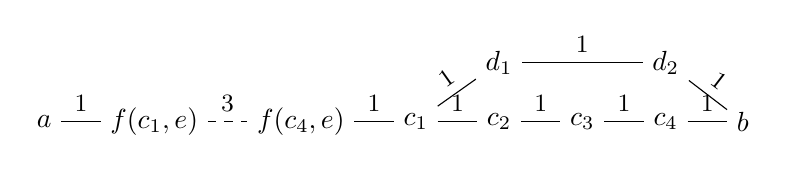
\begin{tikzpicture}[node distance=1.5cm]

\node(a){$a$};

\node(f1)[right = .5cm of a]{$f(c_1,e)$};

\node(f2)[right = .5cm of f1]{$f(c_4,e)$};

\node(c1)[right = .5cm of f2]{$c_1$};

\node(c2)[right = .5cm of c1]{$c_2$};

\node(c3)[right = .5cm of c2]{$c_3$};

\node(c4)[right = .5cm of c3]{$c_4$};

\node(b)[right = .5cm of c4]{$b$};

\node(d1)[above = .25cm of c2]{$d_1$};

\node(d2)[above = .25cm of c4]{$d_2$};

\draw (a) -- (f1)  node [midway, above, sloped] {\small{1}};

\draw (f1) -- (f2) [-,dashed] node [midway, above, sloped] {\small{3}};

\draw (f2) -- (c1) node [midway, above, sloped] {\small{1}};

\draw (c1) -- (c2) node [midway, above, sloped] {\small{1}};

\draw (c2) -- (c3) node [midway, above, sloped] {\small{1}};

\draw (c3) -- (c4) node [midway, above, sloped] {\small{1}};

\draw (c4) -- (b) node [midway, above, sloped] {\small{1}};

\draw (c1) -- (d1) node [midway, above, sloped] {\small{1}};

\draw (d1) -- (d2) node [midway, above, sloped] {\small{1}};
  
\draw (d2) -- (b) node (test) [midway, above, sloped] {\small{1}};

\end{tikzpicture}

\caption{Short explanation example}
\label{fig:short_expl}
\end{figure}

\label{ex:short_expl}
\end{example}

\begin{algorithm}[h]
\caption[.]{insert (Equation Graph)}
  \KwIn{term $s$}
	\KwIn{term $t$}
	\KwIn{extended equality $eq \in \mathcal{E}$}
	%\KwIn{equation graph $g$}
	
	\eIf{$eq \neq \smiley$}{
		add edge $(s,eq,t,1)$ % to $g$
	}
	{
		$f(a,b) \leftarrow s$ \\
		$f(c,d) \leftarrow t$ \\
		$p1 \leftarrow $ shortest path between $a$ and $c$ \\% in $g$ \\
		$p2 \leftarrow $ shortest path between $b$ and $d$ \\% in $g$ \\
		$w \leftarrow \#(p1.inputEqs \cup p2.inputEqs) $ \\
		add edge $(s,\smiley,t,w)$ % to $g$
	}
  
  \label{algo:insert_dij}
\end{algorithm}


\begin{algorithm}[h]
\caption[.]{explain (Equation Graph)}
  \KwIn{term $s$}
	\KwIn{term $t$}
	%\KwIn{equation graph $g$}
	\KwOut{path between $s$ and $t$}
	
	\Return shortest path between $s$ and $t$ found by modified Dijkstra algorithm %in $g$
	
  \label{algo:explain_dij}
\end{algorithm}



\FloatBarrier

\subsubsection*{Proof Forest}

A proof forest is a collection of proof trees.
A proof tree is a labeled tree with nodes in $\mathcal{T}$ and edge labels in $\mathcal{E}$.
For every congruence class in a congruence structure, there is one proof tree.
Inserting an edge between nodes $s$ and $t$ of different proof trees is done by making one the child of the other.
To maintain a tree structure, all edges between the new child and the root of its old tree are reversed.
To limit the number of edge reversion steps, the smaller tree is always attached to the larger one.
This results in $O(n \log(n))$ edge reversion steps, where $n$ is the number terms in the input equation set.
This bound can be shown using the same argument as in the proof of Proposition \ref{prop:runtime}.
As stated above, we understand a path as a sequence of undirected edges.
In case of a proof tree, a path between $s$ and $t$ of the same tree is the combined sequence of edges between the nodes and their nearest common ancestors.
The structure, up to small changes, was proposed in \cite{Nieuwenhuis2005,Nieuwenhuis2007}.
Its benefit is the quick access of explanations and good overall runtime.
Its downside is its inflexibility when it comes to producing alternative explanations.
In fact the explanation returned is always the first one to occur during edge insertion.
The authors of \cite{Nieuwenhuis2005,Nieuwenhuis2007} improve the structure for the special case of flattened terms, for which no term has nesting depth greater than one.

\begin{algorithm}[h]
\caption[.]{insert (Proof Forest)}
  \KwIn{term $s$}
	\KwIn{term $t$}
	\KwIn{extended equation $eq \in \mathcal{E}$}
	%\KwIn{proof forest $g$}
	
	\If{$s$ is not in the graph}{
		add tree with single node $s$ %to $g$
	}
	\If{$t$ is not in the graph}{
		add tree with single node $t$ %to $g$
	}
	
	$sSize \leftarrow $ size of tree of $s$ \\ %in $g$ \\
	$tSize \leftarrow $ size of tree of $t$ %in $g$
	
	\eIf{$sSize \leq tSize$}{
		$(u,v) \leftarrow (s,t)$
	}{
		$(u,v) \leftarrow (t,s)$
	}

	reverse all edges on the path between $u$ and its root node \\
	insert edge $(v,eq,u)$% into $g$

  \label{algo:insert_pt}
\end{algorithm}


\begin{algorithm}[h]
\caption[.]{explain (Proof Forest)}
  \KwIn{term $s$}
	\KwIn{term $t$}
	%\KwIn{proof forest $g$}
	\KwOut{path between $s$ and $t$}
	
	%\eIf{$s$ and $t$ are in the same proof tree $P$}{
		Let $nca$ be the nearest common ancestor of $s$ and $t$ in $P$\\
		$p1 \leftarrow $ path from $s$ to $nca$ \\
		$p2 \leftarrow $ path from $nca$ to $s$ \\
		\Return $p1 :: p2$
	%}{
		%\Return the empty path
	%}

  \label{algo:explain_pt}
\end{algorithm}




\begin{example}

Consider again the set of equations presented in Figure \ref{fig:short_expl} and Example \ref{ex:short_expl} and suppose that the equations $(c_1,d_1),(d_1,d_2),(d_2,b)$ are inserted into the congruence structure before any other equation.
After adding these three equations, the proof forest contains of a single proof tree and is displayed in Figure \ref{fig:proof_forest_1}, where the labels are omitted.
Suppose that now the following equations are inserted: $(a,f(c_1,e)),(f(c_4,e),c_1),(c_1,c_2),(c_2,c_3)$.
The resulting proof forest contains two proof trees and is shown in Figure \ref{fig:proof_forest_2}.
Finally the equation $(c_3,c_4)$ is added and the equality $f(c_1,e) \thickapprox f(c_4,e)$ is deduced.
At this point, the explanation for $c_1 \thickapprox c_4$ in the proof forest is the path $\langle c_1,c_2,c_3,c_4 \rangle$, which is the combined path from $c_1$ and $c_4$ to their nearest common ancestor, which is $c_2$.
The resulting proof forest is shown in Figure \ref{fig:proof_forest_3}, where the explanation for the edge $(f(c_1,e),f(c_4,e))$ is highlighted in a dotted rectangle.
The explanation for $a \thickapprox b$ in this graph is the path $\langle b,d_2,d_1,c_1,f(c_4,e),f(c_1,e),a\rangle$ and since the edge $(f(c_1,e),f(c_4,e))$ uses all other equations as explanation, the final explanation includes all eight equations.
In example \ref{ex:short_expl} we have shown that this is not necessary.

\begin{figure}[ht]

\centering
\begin{tikzpicture}[node distance=1cm]



\node(d1){$d_1$};

\node(c1)[below left=of d1]{$c_1$};

\node(d2)[below right= of d1]{$d_2$};

\node(b)[below= of d2]{$b$};

\draw [->] (c1) -- (d1);% node [midway, above, sloped] {\small{1}};

\draw [->] (d2) -- (d1);% node [midway, above, sloped] {\small{1}};
  
\draw [->] (b) -- (d2);% node (test) [midway, above, sloped] {\small{1}};

\end{tikzpicture}

\caption{Proof Forest including first three equations}
\label{fig:proof_forest_1}
\end{figure}

\begin{figure}[ht]

\centering
\begin{tikzpicture}[node distance=1cm]

\node(c2){$c_2$};

\node(c3)[below left=of c2]{$c_3$};

\node(c1)[below right=of c2]{$c_1$};

\node(t1)[below left=of c1]{$f(c_4,e)$};

\node(d1)[below right=of c1]{$d_1$};

\node(d2)[below= of d1]{$d_2$};

\node(b)[below= of d2]{$b$};

\node(t2)[right =of c2,xshift=2cm]{$f(c_1,e)$};

\node(a)[below =of t2]{$a$};

\draw [->] (c3) -- (c2);
\draw [->] (d1) -- (c1);
\draw [->] (c1) -- (c2);
\draw [->] (d2) -- (d1);
\draw [->] (b) -- (d2);
\draw [->] (t1) -- (c1);

\draw [->] (a) -- (t2);

\end{tikzpicture}

\caption{Proof Forest before deducing}
\label{fig:proof_forest_2}
\end{figure}

\begin{figure}[ht]

\centering
\begin{tikzpicture}[node distance=1cm]
\node(t1){$f(c_4,e)$};

\node(c1)[below =of t1]{$c_1$};

\node(c2)[below of=c1]{$c_2$};

\node(c3)[below =of c2]{$c_3$};

\node(c4)[below =of c3]{$c_4$};

\node(d1)[below right=of c1]{$d_1$};

\node(d2)[below= of d1]{$d_2$};

\node(b)[below= of d2]{$b$};

\node(t2)[below left=of t1]{$f(c_1,e)$};

\node(a)[below =of t2]{$a$};

\node[rectangle,rounded corners,draw,dotted,fit=(c1) (c2) (c3) (c4)](rect) {};

\draw [->] (c4) -- (c3);
\draw [->] (c3) -- (c2);
\draw [->] (d1) -- (c1);
\draw [->] (c2) -- (c1);
\draw [->] (d2) -- (d1);
\draw [->] (b) -- (d2);
\draw [->] (c1) -- (t1);
\draw [->] (t2) -- (t1) node [midway, below] (expl) {};
\draw [->] (a) -- (t2);
\draw [->,dotted] (expl) -- (rect);

\end{tikzpicture}

\caption{Final Proof Forest}
\label{fig:proof_forest_3}
\end{figure}

\end{example}

%See how BarceLogic ppl prove stuff,
%-) tree is still tree after inserting
%-) path to NCA forms explanation


\FloatBarrier

\section{Proof Production}
\label{sec:proofproduction}

In this section we describe how to produce resolution proofs from paths in a congruence graph.
The method to carry out this operation is \texttt{produceProof}.
The basic idea is to traverse the path, creating a transitivity chain of equalities between adjacent nodes, while keeping track of the deduced equalities in the chain.
From Invariant Deduced Edges follows that for the deduced equalities there have to be paths between the respective arguments of the compound terms.
These paths are transformed into proofs recursively and resolved with a suiting instance of the compatibility axiom.
After this operation the subproof is resolved with the original transitivity chain.
Since terms can never be equal to their (proper) subterms, the procedure will eventually terminate.
The result of this procedure is a resolution proof with a root, such that the equations of the negative literals are an explanation of the target equality or $\emptyset$ to denote that the equality can not be proven.
Suppose some equality $s \thickapprox t$ can be explained and \texttt{produceProof} returns a proof with root $\rho$, then it is the case that $neg(\rho) \models s \thickapprox t$ and $neg(\rho)$ is a subset of the input equations.

\begin{algorithm}[t]
\caption[.]{produceProof}
  \KwIn{term $s$}
	\KwIn{term $t$}
	%\KwIn{congruence graph $g$}
	\KwOut{Resolution proof for $E \models s \thickapprox t$ or $\emptyset$}
	
	$p \leftarrow explain(s,t,g)$ \\
	$d \leftarrow \emptyset$ \\
	$e \leftarrow \emptyset$ \\
	
	\While{$p$ is not empty}{
		$(u,l,v) \leftarrow $ first edge of $p$ \\
		$p \leftarrow p \setminus (u,l,v)$ \\
		$e \leftarrow e \cup \{u \neq v\}$ \\
		\If{$l = \smiley$}{
			$f(a,b) \leftarrow u$ \\
			$f(c,d) \leftarrow v$ \\
			$p_1 \leftarrow produceProof(a,c)$ \\
			$p_2 \leftarrow produceProof(b,d)$ \\
			$con \leftarrow \{ a \neq c, b\neq d, f(a,b) = f(c,d) \}$ \\
			$res \leftarrow$ resolve $con$ with non $\emptyset$ roots of $p_1$ and $p_2$ \\
			%$int_1 \leftarrow$ resolve $con$ with $root(p_1)$ \\
			%$int_2 \leftarrow$ resolve $int_1$ with $root(p_2)$ \\
			$d \leftarrow d \cup res$
		}
	}
	
	\If{$\# e > 1$}{
		$proof \leftarrow e \cup \{s = t\}$ \\
		\While{$d$ is not empty}{
			$int \leftarrow $ some element in $d$ \\
			$d \leftarrow d \setminus \{int\}$ \\
			$proof \leftarrow $ resolve $proof$ with $int$
		}
		\Return $proof$
	}
	\ElseIf{$d = \{ded\}$}{
		\Return $ded$
	}
	\Else{
		\If{$e = \{(u,l,u)\}$} {
			\Return $\{u = u\}$
		}
		\Else {
			\Return $\emptyset$
		}
	}
	
  \label{algo:prodproof}
\end{algorithm}



\begin{example}

Consider again the congruence graph shown in Figure \ref{fig:short_expl} and suppose we want a proof for $a \thickapprox b$.
Suppose we found the path $p_1 := \langle  a, f(c_1,e), f(c_4,e), c_1, c_2, c_3, c_4, b \rangle$ as an explanation and that the explanation for $f(c_1,e) \thickapprox f(c_4,e)$ is the path $\langle c_1, c_2, c_3, c_4 \rangle$.
We transform $p_1$ and $p_2$ into instances of the transitivity axiom $C_1$ and $C_2$ respectively. 
The clause $C_2$ is resolved with the instance of the congruence axiom $C_3$, which is then resolved with the instance of the reflexive axiom $C_4$ resulting in clause $C_5$.
Finally, $C_1$ is resolved with $C_5$ to obtain the final clause $C_6$.
The proof is shown in Figure \ref{fig:proofprod}.

\begin{figure}[!h]

\centering
\begin{tikzpicture}[node distance=1.5cm]
	%\proofnode{root} {$a \neq f(c_1,e), f(c_4,e) \neq c_1, c_1 \neq c_2, c_2 \neq c_3, c_3 \neq c_4, c_4 \neq b, a = b$};
	%
	%%\proofnode{root} {$C_6$};
	%
	%\withchildren{root} {c1}{$a \neq f(c_1,e), f(c_1,e) \neq f(c_4,e), f(c_4,e) \neq c_1, c_1 \neq c_2, c_2 \neq c_3, c_3 \neq c_4, c_4 \neq b, a = b$} {c5}{$c_1 \neq c_2, c_2 \neq c_3, c_3 \neq c_4, f(c_1,e) = f(c_4,e)$};
	%
	%\withchildren{c5} {c4}{$e = e$} {tmp}{tmp};
	%
	%\withchildren{tmp} {c3}{$e \neq e, c_1 \neq c_4, f(c_1,e) = f(c_4,e)$} {c2}{$c_1 \neq c_2, c_2 \neq c_3, c_3 \neq c_4, c_1 = c_4$};


	\proofnode[xshift=-1cm,font=\small,align=center]{root} {$C_6$\\$a \neq f(c_1,e), f(c_4,e) \neq c_1, c_1 \neq c_2, c_2 \neq c_3, c_3 \neq c_4, c_4 \neq b, a = b$};
	
	\proofnode[above left of=root,yshift=1.25cm,xshift=-2.75cm,align=center,font=\small]{c1}{$C_1$\\$a \neq f(c_1,e), f(c_1,e) \neq f(c_4,e), f(c_4,e) \neq c_1,$\\$ c_1 \neq c_2, c_2 \neq c_3, c_3 \neq c_4, c_4 \neq b, a = b$};
	\proofnode[above right of=root,yshift=.5cm,xshift=2cm,align=center,font=\small]{c5}{$C_5$\\$c_1 \neq c_2, c_2 \neq c_3, c_3 \neq c_4, f(c_1,e) = f(c_4,e)$};

	\proofnode[above left of=c5,xshift=-1.5cm,align=center,font=\small]{c4}{$C_4$\\$e = e$};
	\proofnode[above right of=c5,xshift=1cm,align=center,font=\small]{tmp}{$e \neq e, c_1 \neq c_2, c_2 \neq c_3, c_3 \neq c_4, f(c_1,e) = f(c_4,e)$};

	\proofnode[above left of=tmp,align=center,xshift=-2.5cm,font=\small]{c3}{$C_3$\\$e \neq e, c_1 \neq c_4, f(c_1,e) = f(c_4,e)$};
	\proofnode[above right of=tmp,align=center,yshift=1cm,xshift=-.75cm,font=\small]{c2}{$C_2$\\$c_1 \neq c_2, c_2 \neq c_3, c_3 \neq c_4, c_1 = c_4$};

	\drawchildren{root}{c1}{c5};
	\drawchildren{c5}{c4}{tmp};
	\drawchildren{tmp}{c3}{c2};
	
	%\proofnode[right of=root, xshift=2cm]{root2} {$t_a \neq a, a\neq b, b \neq t_b, t_a = t_b$};
	
\end{tikzpicture}


\caption{Example proof}
\label{fig:proofprod}
\end{figure}

\end{example}

As mentioned in Section \ref{sec:congruenceclosurealgorithm}, edges are inserted into a congruence graph in a lazy way by the congruence closure algorithm.
The reason is that \texttt{produceProof} searches for explanations for edges with label $\smiley$.
Should the equality of question be an input equation that is added later to the congruence structure than it was deduced, then we would like to overwrite this label with the input equation.
The impact of lazy insertion gets larger, if an implementation searches for explanations already when an edge is added to the graph.
Example \ref{example:lazy} shows how this technique can help producing shorter proofs.

\begin{example}
\label{example:lazy}
Suppose we want to add the following sequence of equations into an empty congruence structure: $\langle (a,b),(f(a,a),d),(f(b,b),e),(f(a,a),f(b,b)) \rangle$.
After adding the first three equations, the congruence closure algorithm detects the deduced equality $f(a,a) \thickapprox f(b,b)$.
The explanation for this equality is $\{(a,b)\}$, if we were to insert the edge $(f(a,a),f(b,b))$ into the graph immediately, it would have weight 1 and label $\smiley$.
Depending on the congruence graph used, when adding the fourth equation $(f(a,a),f(b,b))$ to the congruence structure, either the edge $(f(a,a),f(b,b))$ is not added at all to the graph or is added with weight 1.
In the latter case, both edges have weight 1 and equal chance to be selected by the shortest path algorithm.
However, choosing the edge with label $\smiley$ is undesirable, since it two extra resolution nodes (corresponding to the compatability axiom and an intermediate node).

\end{example}

\FloatBarrier

\subsection*{Congruence Compressor}

In this section we put our explanation producing congruence closure algorithm and the proof production method into the context of proof compression.
To this end we replace subproofs with conclusions that contain unnecessary long explanations with new proofs that have shorter conclusions.
Shorter conclusions lead to less resolution steps further down the proof and possibly large chunks of the proof can simply be discarded.
There is however a tradeoff in overall proof length when introducing new subproofs.
The subproof corresponding to a short explanation can be longer in proof length, i.e. involve more resolution nodes, than one with a longer explanation.
Example \ref{example:shortexpl} displays this issue.
Additionally it can be the case that by introducing a new subproof, we only partially remove the old subproof.
Some nodes of the old subproof might still be used in other parts of the proof.
Therefore the replacement of a subproof by another, smaller one does not necessarily lead to a smaller proof.
Nevertheless, our intuition is that favoring smaller conclusions should dominate such effects, especially on large proofs.

%In Section \ref{sec:proofprocessing} processing of a proof was defined.
%The most important application of proof processing for this work is proof compression.

\begin{example}
\label{example:shortexpl}
For presentation purposes, throughout this example we will abbreviate the term $f(f(a,b),f(a,a))$ with $t_a$ and $f(f(b,a),f(b,b))$ with $t_b$.
Consider the set of equations $E = \{(t_a,a),(a,b),(b,t_b)\}$ and the target equality $t_a \thickapprox t_b$.
Using equations in $E$, one can prove the the target equality in two ways.
Either one uses the instance of the transitivity axiom $\{t_a \neq a, a \neq b, b \neq t_b, t_a = t_b\}$ or a repeated applications of instances of the congruence axiom, e.g. $\{a \neq b, f(a,a) = f(b,b)\}$.
The corresponding explanations are $E$ and $\{(a,b)\}$.

The two resulting proofs are shown in Figure \ref{fig:short_expl_proof}.
The proof with the longer explanation $E$ is only one proof node, whereas the proof with the singleton explanation has proof length 5.

\begin{figure}[!h]

\centering
\begin{tikzpicture}[node distance=2.5cm]
	\proofnode[align=center]{root} {$a \neq b, t_a = t_b$\\Congruence proof};
	
	\proofnode[above left of=root,yshift=.25cm]{n5}{$a \neq b, f(a,a) \neq f(b,b), t_a = t_b$};
	\proofnode[above right of=root,yshift=-.25cm]{n7}{$a\neq b, f(a,a) = f(b,b)$};

	\proofnode[above left of=n5,yshift=.25cm]{n3}{$f(a,b) \neq f(b,a), f(a,a) \neq f(b,b), t_a = t_b$};
	\proofnode[above right of=n5,yshift=-.25cm]{n4}{$a \neq b, f(a,b) = f(b,a)$};

	\drawchildren{root}{n5}{n7};
	\drawchildren{n5}{n3}{n4};
	
	\proofnode[right of=root, xshift=2cm, align=center]{root2} {$t_a \neq a, a\neq b, b \neq t_b, t_a = t_b$\\Transitivity proof};
\end{tikzpicture}


\caption{Short explanation, long proof}
\label{fig:short_expl_proof}
\end{figure}

\end{example}

The Congruence Compressor compresses processes a proof replacing subproofs as described above. 
It is defined upon the processing function $f: V \times V \times V \rightarrow V$ specified in pseudocode in Algorithm \ref{algo:compressor}.
The function $g_f: V \rightarrow V$ for axioms is simply the identity (i.e. axioms are not modified).
The idea of the processing function is simple.
Axioms are not changed by the function.
For all other nodes the \texttt{fixNode} method is called, to maintain a correct proof.
For a clause $C$, the method adds $neg(C)$ (as defined in \ref{sec:calculus}) to the empty congruence structure and checks whether these equations induce a proof for one of the equations in the $pos(C)$ that has a shorter conclusion than the original subproof.
If there is such a proof, we replace the old subproof by the new one.
Example \ref{example:compressproof} displays this procedure.

In line \ref{criteria} it is decided whether the explanation finding congruence closure algorithm should be used to find a replacement for the current node.
A trivial criteria is true for every node.
Testing every node will result in a slow algorithm, but the best possible compression.
Some nodes do not need to be checked, since they contain optimal explanations by definition or there is no hope of finding an explanation at all.
The following definition classifies nodes to define a more sophisticated decision criteria.

\begin{definition}[Types of nodes]

An axiom is a \emph{theory lemma} if it is an instance of one of the congruence axioms.
Otherwise it is \emph{input derived}.
The classification of internal nodes is defined recursively.
An internal node is input derived, if one of its premises is input derived.
Otherwise it is a theory lemma.
We call a node a \emph{low theory lemma} if it is a theory lemma and has a child that is input derived.

\end{definition}

We suspect that most redundancies in proofs are to be found in low theory lemmas, since they reflect the explanations found by the proof producing solver.
Therefore an alternative criteria is to only find replacements for low theory lemmas.
The question whether a node is a low theory lemma is not trivial to answer while traversing the proof in a top to bottom fashion.
Therefore a preliminary traversal is necessary to determine the classification of nodes.
%Experiments have shown that using this criteria speeds up the algorithm a lot, while losing only very little compression.
Further criteria for deciding whether or not to replace could be size of the subproof or a global metric that tries to predict the global compression achieved by replacement.

\begin{algorithm}[h]
\caption[.]{compress}
	\KwGlobal{set of input equations $E$}
	\KwIn{resolution node $n$}
  \KwIn{$pr:$ tuple of resolution nodes $(p_1,p_2)$}
	\KwOut{resolution node}

	$m \leftarrow fixNode(n,(p_1,p_2))$ \\
	\If{$m$ fulfills criteria \label{criteria}}{
		$lE \leftarrow \{(a,b) \mid (a \neq b) \in m\}$ \\
		$rE \leftarrow \{(a,b) \mid (a = b) \in m\}$ \\
		$con \leftarrow $ empty congruence structure \\
		\For{$(a,b)$ in $lE$}{
			$con \leftarrow con.addEquality(a,b)$
		}
		\For{$(a,b)$ in $rE$}{
			$con \leftarrow con.addNode(a).addNode(b)$ \\
			$proof \leftarrow con.prodProof(s,t)$ \\
			\If{$proof \neq \emptyset$ and $| proof.conclusion | < | m.conclusion |$}{
				$m \leftarrow proof$
			}
		}
	}
	\Return $m$
  \label{algo:compressor}
\end{algorithm}


The compressor (Algorithm \ref{algo:compressor}) uses the method \texttt{fixNode} to maintain a correct proof.
The method modifies nodes with premises that have earlier been replaced by the compressor. 
Nodes with unchanged premises are not changed.
Let $n$ be a proof node that was derived using pivot $\ell$ in the original proof and which updated premises are $pr_1$ and $pr_2$ .
Depending on the presence of $\ell$ in $pr_1$ and $pr_2$, $n$ is either replaced by the resolvent of $pr_1$ and $pr_2$ or by one of the updated premises.
In case both updated premises do not contain the original pivot element, replacing the node by either one of them maintains a correct proof.
Since we are interested in short proofs, we return the one with the shorter clause.
This method of maintaining a correct proof was proposed in \cite{Bar-Ilan2008} in the context of similar proof compression algorithms.

\begin{algorithm}[h]
\caption[.]{fixNode}
	\KwIn{resolution node $n$}
  \KwIn{$pr:$ tuple of resolution nodes $(p_1,p_2)$}
	\KwOut{resolution node}
	
	\eIf{($n.premise_1 = p_1$ and $n.premise_2 = p_2$)}{
		\Return $n$
	}{
		\If{$n.pivot \in p_1$ and $n.pivot \in p_2$}{
			\Return $resolve(p_1,p_2)$
		}
		\ElseIf{$n.pivot \in p_1$}{
			\Return $p_2$
		}
		\ElseIf{$n.pivot \in p_2$}{
			\Return $p_1$
		}
		\Else{
			\Return node with smaller clause
		}
	}

  \label{algo:fixnode}
\end{algorithm}



\begin{example}
\label{example:compressproof}
Consider the proof presented graphically in Figure \ref{fig:compressproof}.
It uses the same abbreviations for $t_a$ and $t_b$ as in Example \ref{example:shortexpl}.
Furthermore, the proof uses the long explanation for $t_a \thickapprox t_b$.
The length of the proof is 12.
The proof contains one propositional variable $A$.
The compression algorithm traverses the proofs and detects the redundant explanation in node $O_1$.
The subproof $N_1$ corresponding to the explanation $\{(a,b)\}$ is created and $O_1$ is replaced by it.
The construction of this subproof is discussed in Example \ref{example:shortexpl}.
When iterating over node $O_2$, the algorithm detects that the pivot literal $t_a = a$ is not present in $N_1$ and \texttt{fixNode} replaces $O_2$ by $N_1$.
At node $O_3$, both premises contain the pivot $a = b$, therefore $O_3$ is replaced by resolvent of $N_1$ and its other original premise.
No other subproof is altered by the algorithm.
The resulting proof is displayed in Figure \ref{fig:compressproof_2} and has length 11 which is shorter than the original one, even though the replaced subproof is larger.
Note that the clause $\{\neg A\}$ is part of the replaced subproof.
It is also part of the subproof with conclusion $\{a = b\}$, which remains in the new proof.

\begin{figure}[!h]

\centering
\begin{tikzpicture}[node distance=2.5cm]

	\rootnode;
	
	\withchildren{root}{n11}{$t_a = t_b$} {n10}{$t_a \neq t_b$};

	\proofnode[above left of=n11, align=center,font=\small]{n9}{$b \neq t_b$};
	\proofnode[above right of=n11, align=center,font=\small]{n8}{$O_3$\\$b \neq t_b, t_a = t_b$};
	\drawchildren{n11}{n9}{n8};
	\proofnode[above left of=n8, align=center,font=\small]{n5}{$O_2$\\$a \neq b, b\neq t_b, t_a = t_b$};
	
	\proofnode[above left of=n5, align=center,font=\small]{n1}{$O_1$\\$t_a \neq a, a\neq b, b \neq t_b, t_a = t_b$};
	\proofnode[above right of=n5]{n4}{$t_a = a$};
	\drawchildren{n5}{n1}{n4};
	\proofnode[above left of=n4]{n2}{$A,t_a = a$};
	
	
	
	\proofnode[right of =n4]{n7}{$a = b$};
	\drawchildren{n8}{n5}{n7};
	\withchildren{n7}{n3}{$\neg A$} {n6}{$A, a = b$};
	\drawchildren{n4}{n2}{n3};
\end{tikzpicture}


\caption{Original Proof}
\label{fig:compressproof}
\end{figure}

\begin{figure}[!h]

\centering
\begin{tikzpicture}[node distance=2.5cm]
	
	
	\rootnode;
	
	\withchildren{root}{new9}{$t_a = t_b$} {new10}{$t_a \neq t_b$};
	
	\proofnode[above right of=new9,yshift=-1cm,xshift=.5cm]{new8}{$a = b$};

	\proofnode[above left of=new9, align=center,font=\small]{new5} {$N_1$\\$a \neq b, t_a = t_b$};
	
	\proofnode[above left of=new5,yshift=.25cm]{n5}{$a \neq b, f(a,a) \neq f(b,b), t_a = t_b$};
	\proofnode[above right of=new5,yshift=-.25cm]{n7}{$a\neq b, f(a,a) = f(b,b)$};

	\proofnode[above left of=n5,yshift=.25cm]{n3}{$f(a,b) \neq f(b,a), f(a,a) \neq f(b,b), t_a = t_b$};
	\proofnode[above right of=n5,yshift=-.25cm]{n4}{$a \neq b, f(a,b) = f(b,a)$};

	\drawchildren{new5}{n5}{n7};
	\drawchildren{n5}{n3}{n4};
	
	\drawchildren{new9}{new5}{new8};
	
	\withchildren{new8}{new6}{$\neg A$} {new7}{$A,a = b$};
\end{tikzpicture}


\caption{Compressed Proof}
\label{fig:compressproof_2}
\end{figure}

\end{example}

\FloatBarrier


\section{Experiments}
\label{sec:congruence_experiments}

In this section, we present the experimental evaluation of our length compression algorithm.
We tested our method on 3965 proofs of problems of the SMT-LIB benchmark.
The proofs were created from problems in the SMT theory QF\_UF, which is the logic of unquantified formulas built over a signature of uninterpreted (i.e. free) sort and function symbols\footnote{QF\_UF specification: \url{http://smtlib.cs.uiowa.edu/logics/QF\_UF.smt2}}, using the SMT solver VeriT \cite{Bouton2009}.
The average length of the proofs is 103450 nodes and the largest proof has length 2241042.

We evaluated the compression achieved by our algorithm for the two different Congruence Graph structures, presented in Section \ref{sec:algorithm}.
We post processed the produced proofs with another compression algorithm called DAGify.
DAGify traverses the proofs and merges duplicate nodes.
This was necessary, because our the congruence compression algorithm creates the same axioms and intermediate nodes multiple times.
A future version of our algorithm should keep track of and reuse nodes, so the post processing is not necessary.
To present unbiased results, we also compressed the proofs with DAGify to show how much of the compression is achieved by this method.

The compression results are presented in Table \ref{tab:congruence_results}, where the rows Equation Graph and Proof Forest display the results of our congruence compression algorithm using the respective type of Congruence Graph.
The row DAGify displays the compression achieved by this algorithm.
\textbf{Compression} was calculated according to Formula \ref{eq:length}, where $f$ is the respective compression algorithm and $B$ denotes the set of benchmark proofs.
The columns \textbf{Min}- and \textbf{Max Compression} show the minimum and maximum compression ratio achieved by the algorithms.
On top of compression, we measure computation speed measured in processed nodes per millisecond.
The best respective results are highlighted in boldface.

\begin{align}
	compression(f) = 1 - \frac{\sum_{\varphi \in B}{\plength{f(\varphi)}}}{\sum_{\varphi \in B}{\plength{\varphi}}}
  \label{eq:length}
\end{align}


%%%%%%%%%%%%%%%%%%%%%%%%%%%%%%%%%%%%%%%%%%%%%%%%%%%%%%%%%%%%%%
%%%%%%%%%%%%%%% Results table %%%%%%%%%%%%%%%%%%%%%%%%%%%%%%%%
%%%%%%%%%%%%%%%%%%%%%%%%%%%%%%%%%%%%%%%%%%%%%%%%%%%%%%%%%%%%%%

\begin{table}[h]
\centering
%\setlength{\tabcolsep}{8pt}
\begin{tabular}{l c c c c}
\toprule
\textbf{Method} & \textbf{Compression} & \textbf{Min Compression} & \textbf{Max Compression} & \textbf{Speed}\\ 
\midrule

Equation Graph & \textbf{5.350} \% & -18.302 \% & \textbf{81.347} \% & 0.343 \\ 
Proof Forest &  5.196 \% & -43.985 \% & 77.202 \% & 0.611 \\ 
DAGify & 3.368 \% & \textbf{0.0} \% & 14.433 \% & \textbf{1.655} \\ 

\bottomrule
%\hline
\end{tabular}
\caption{Compression Results}
\label{tab:congruence_results}
\end{table}

The compression results presented in Table \ref{tab:congruence_results} show that our compression algorithm can achieve an effective compression of roughly 2\%.
This is not really a satisfying number, but the maximum compression for single proofs shows, that our algorithm can perform very well on some examples.
The min compression column shows, that sometimes our method increases the proof length.
However, as seen in Figure \ref{fig:congruence_compression}, this only happens for small proofs.
Figure \ref{fig:congruence_compression} displays the compression achieved by our algorithm, using the Equation Graph data structure, in relation to the proof length.
Every point in the plot represents a proof, where the x-coordinate is its length and the y-coordinate denotes the compression achieved on this proof.
The plot shows that our algorithm has the trend to produce better compression on larger proofs and those are the proofs that are especially interesting for proof compression and in general.

\begin{figure}[h]
	\centering
	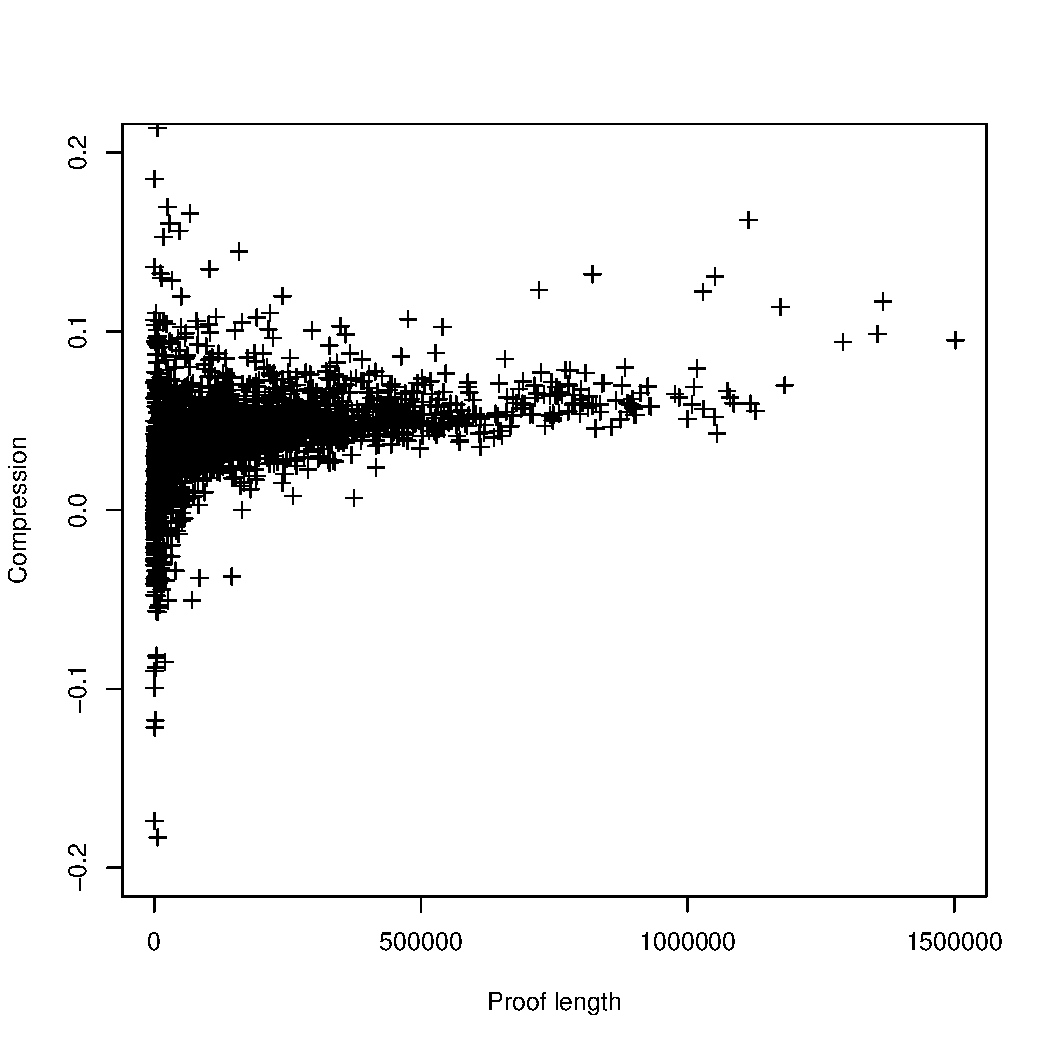
\includegraphics[scale=0.8]{figures/compression_vs_length.pdf}
	\caption{Compression vs Proof Length}
	\label{fig:congruence_compression}
\end{figure}

In Section \ref{sec:proofproduction}, we discussed the question on which proof nodes the congruence closure algorithm should be applied to.
For the results presented, the algorithm has been applied to all nodes.
Preliminary experiments showed unpromising results, when the compression algorithm is only applied to low theory lemmas.
A reason could be that the original proofs resolve with input derived nodes early.
The result of such a resolving strategy is that the explanation for some equation is split into multiple nodes or in an input derived node.
In other words, a proof that fulfills the assumption stated in the proof of Proposition \ref{prop:extended_resolution} should contain all explanations in a low theory lemma.
However, proofs created by VeriT do not satisfy this assumption.
Therefore, taking into account equations of ancestor nodes for an explanation in the compression algorithm could improve performance.

On top of proof compression, we measured the explanation sizes produced using the two types Congruence Graphs.
The results are displayed in Table \ref{tab:explanation_results}.
Overall 6604751 explanations were produced by each congruence graph structure.
Of the nodes corresponding to these explanations, 5114638 (77.439 \%) are theory lemmas and 1710435 (25.897\%) are low theory lemmas.
The column \textbf{Compressed} shows the percentage of explanations produced by our algorithm that are strictly smaller than the ones present in the proof.
Note that the produced explanations are at most as large as the original ones by design of the method.
Among the compressed explanations explanations, the column \textbf{Compression} shows the compression ratio achieved, computed according to $1 - \frac{\text{produced}}{\text{original}}$.

%%%%%%%%%%%%%%%%%%%%%%%%%%%%%%%%%%%%%%%%%%%%%%%%%%%%%%%%%%%%%%
%%%%%%%%%%%%%%% Explanation table %%%%%%%%%%%%%%%%%%%%%%%%%%%%
%%%%%%%%%%%%%%%%%%%%%%%%%%%%%%%%%%%%%%%%%%%%%%%%%%%%%%%%%%%%%%

\begin{table}[h]
\centering
%\setlength{\tabcolsep}{8pt}
\begin{tabular}{l c c}
\toprule
\textbf{Congruence Graph} & \textbf{Compressed} & \textbf{Compression} \\ 
\midrule

Equation Graph & 12.42 \% & 28.34 \% \\ 
Proof Forest & 11.459 \% & 28.69 \% \\ 

\bottomrule
%\hline
\end{tabular}
\caption{Explantion Size Results}
\label{tab:explanation_results}
\end{table}

The results show that our explanation producing congruence closure algorithm is able to produce shorter explanations than those of the benchmark proofs often.
The two data structures do not show very significant performance differences and the 1 \% more compressed explanations explain the slight performance edge in proof compression of the Equation Graph over the Proof Forest.

It is surprising that a significant amount of explanations could be compressed by a significant percentage, but still the proof compression achieved is rather small.
The reason probably lies in our proof producing algorithm that produces redundant proofs in some other characteristic than explanation size.
Another reason probably is the combination of fragments of the original proof and newly produced subproofs.
In Section \ref{sec:proofproduction} and Example \ref{example:compressproof} we briefly discussed nodes remaining in the proof when replacing subproofs.
This effect seems to be significant.

However, the results also show that using our congruence closure algorithm within the proof production process in the first place will produce proofs that are even shorter than the ones we are able to obtain by compressing them after creation.
Furthermore, the algorithm can be used in other context where small explanations are desired.

\subsection{Future Work}

\cite{Bachmair2000} compares the running times of several congruence closure algorithms.
It would be interesting to do a similar comparison including the congruence closure algorithm presented in Section \ref{sec:algorithm}.
A comparison to the classic congruence closure algorithms of Nelson and Oppen \cite{Nelson1980}, Downey, Sethi and Tarjan \cite{Downey1980} and Shostak \cite{Shostak1978} and their abstract counterparts, as described in \cite{Bachmair2000}, would show whether our method can compete in terms of computation speed.
Comparing our method with the explanation producing algorithms presented in \cite{Fontaine2004} and \cite{Nieuwenhuis2005,Nieuwenhuis2007} could be done not only in terms of speed, but also in terms of explanation size.

In Section \ref{sec:npcomplete} it was shown that the problem of finding the shortest explanation is NP-complete.
Therefore further methods and heuristics to find short explanations could be investigated.
The idea of using shortest path algorithms for explanation finding is a step in that direction.
In \ref{sec:algorithm} we describe a modification of Dijkstra's algorithm \cite{Dijkstra1959} to make it sensitive to previously used equations.
Further modifications, possibly using heuristics, could lead to a short explanation algorithm.
Furthermore translating the problem into a SAT instance could result in an algorithm to derive shortest explanations in acceptable time.

The congruence closure algorithm could be implemented into a SMT solver.
Such solvers usually have high requirements regarding computation time.
It would be interesting to see, whether the method presented in this work can match these requirements.

\cite{Nieuwenhuis2007} extends the congruence closure algorithm to the theory of integer offsets.
Such an extension to our algorithm would be interesting.
Not only could more proofs be compressed, but also the compression ratio on the current benchmarks would increase.

In Section \ref{sec:congruence_experiments}, we compare our method only to proofs produced by the solver VeriT.
Comparing to proofs of other solvers would provide a bigger picture of how well our compression and explanation production algorithms perform.

The use of immutable data structures in the congruence closure algorithm allows to easily keep track of a collection of congruence structures for different sets of input equations.
When the congruence structure of some set of equations is required, it does not necessarily have to be constructed from scratch, but a previously constructed congruence structure, that has a subset of the input equations inserted, could be extended.
Using this technique would speed up the whole method.

\bibliographystyle{plain}
\bibliography{jabref_references}

\end{document}

